\documentclass[10pt,a4paper]{article}
\usepackage[paper=a4paper, hmargin=1.5cm, bottom=1.5cm, top=3cm]{geometry}

\usepackage[utf8x]{inputenc}
\usepackage[spanish]{babel}

\usepackage{mathtools}
\usepackage{amsmath}
\usepackage{amsfonts}
\usepackage{amssymb}

\usepackage{xcolor}
\usepackage{listingsutf8}
\usepackage{booktabs}
\usepackage{hyperref}

\usepackage{caption}
\usepackage{subcaption}

\usepackage{algorithm}
\usepackage[noend]{algpseudocode}

\usepackage{graphicx}
\usepackage{tikz}
\usepackage{relsize}

\usepackage{chessboard}
\storechessboardstyle{6x6}{maxfield=h8}

\DeclarePairedDelimiter{\ceil}{\lceil}{\rceil}

%\let\NombreFuncion=\textsc
%\let\TipoVariable=\texttt

%\newcommand{\TipoFuncion}[3]{%
  %\NombreFuncion{#1}(#2) \ifx#3\empty\else $\to$ \res\,: \TipoVariable{#3}\fi%
%}

% set the default code style
\lstset{
    frame=tb, % draw a frame at the top and bottom of the code block
    tabsize=4, % tab space width
    showstringspaces=false, % don't mark spaces in strings
    numbers=left, % display line numbers on the left
    commentstyle=\color{green}, % comment color
    keywordstyle=\color{blue}, % keyword color
    stringstyle=\color{red} % string color
}

% mathy stuff
\newtheorem{theorem}{Theorem}[section]
\newtheorem{lemma}[theorem]{Lemma}
\newtheorem{proposition}[theorem]{Proposición}
\newtheorem{corollary}[theorem]{Corollary}

\newenvironment{proof}[1][Demostración]{\begin{trivlist}
\item[\hskip \labelsep {\bfseries #1}]}{\end{trivlist}}
\newenvironment{definition}[1][Definición]{\begin{trivlist}
\item[\hskip \labelsep {\bfseries #1}]}{\end{trivlist}}
\newenvironment{example}[1][Example]{\begin{trivlist}
\item[\hskip \labelsep {\bfseries #1}]}{\end{trivlist}}
\newenvironment{remark}[1][Remark]{\begin{trivlist}
\item[\hskip \labelsep {\bfseries #1}]}{\end{trivlist}}

\newcommand{\qed}{\nobreak \ifvmode \relax \else
      \ifdim\lastskip<1.5em \hskip-\lastskip
      \hskip1.5em plus0em minus0.5em \fi \nobreak
      \vrule height0.75em width0.5em depth0.25em\fi}

\title{Algoritmos y Estructuras de Datos III \\ TP3}

\newcommand{\order}[1]{$\mathcal{O}(#1)$}

\begin{document}

%% cover page

\maketitle

\bigskip

\begin{table}[h]
\centering
\begin{tabular}{|l l l|}
\hline
Integrante       & \multicolumn{1}{c}{LU}     & Correo electrónico        \\ \hline
Martin Baigorria & \multicolumn{1}{c}{575/14} & martinbaigorria@gmail.com \\ 
Federico Beuter & 827/13                      & federicobeuter@gmail.com \\
Juan Rinaudo & 864/13                      & jangamesdev@gmail.com \\ 
Mauro Cherubini & 835/13                      & cheru.mf@gmail.com \\ \hline
\end{tabular}
\end{table}

\vfill

\begin{center}
\textbf{Reservado para la cátedra}
\end{center}
\begin{table}[h]
\centering
\begin{tabular}{|l|l|l|}
\hline
Instancia       & Docente & Nota \\ \hline
Primera entrega &         &      \\ \hline
Segunda entrega &         &      \\ \hline
\end{tabular}
\end{table}

\newpage
\tableofcontents
\newpage

% end cover page

\section{Introducción}

\subsection{Definiciones}

Antes de enunciar el problema a resolver en este trabajo practico, es necesario definir algunos conceptos.

Sea $G = (V,E)$ un grafo simple:
\begin{definition}
Un conjunto $I \subseteq V$ es un \textit{conjunto independiente} de $G$ si no existe ningún eje de $E$ entre los vértices de $I$. Es decir, los ejes de $I$ no están conectados por las aristas de $G$.
\end{definition}

\begin{definition}
Un conjunto $D \subseteq V$ es un \textit{conjunto dominante} de G si todo vértice de $G$ esta en $D$ o bien tiene al menos un vecino que esta en $D$.
\end{definition}

\begin{definition}
Un conjunto \textit{conjunto independiente dominante} de $G$ es un conjunto independiente que a su vez es dominante del grafo G. Desde un conjunto independiente dominante se puede acceder a cualquier vértice del grafo $G$ con solo recorrer una arista desde uno de sus vértices.
\end{definition}

\begin{definition}
Un \textit{Conjunto Independiente Dominante Mínimo} (CIDM) es el conjunto independiente dominante de $G$ de mínima cardinalidad.
\end{definition}

Cada definición debería ser acompañada con un gráfico. Por ejemplo, podemos mostrar dos conjuntos independientes y dominantes del mismo grafo, donde uno ese el CIDM.

\subsection{Introducción}
En 1979, Garey y Johnson probaron que el problema de encontrar el CIDM de un grafo es un problema NP-Hard\footnote{M.R. Garey, D.S. Johnson, Computers and Intractability: A Guide to the Theory of NP-Completeness, Freeman and Company, San Francisco (1979).}.
El objetivo del trabajo es utilizar diferentes técnicas algorítmicas para resolver este problema. En un principio diseñaremos e implementaremos un algoritmo exacto para el mismo. Dada la complejidad del problema, luego propondremos diferentes algoritmos heurísticos para llegar a una solución que sea lo suficientemente buena a fines prácticos en un tiempo razonable.

Si recordamos el problema 3 del TP1, podemos ver claramente que el mismo es un caso particular del problema del conjunto independiente dominante optimo. Esto se debe a que el problema de los caballos imponía cierta estructura sobre el grafo en el que se efectuaba la búsqueda. El grafo en si no era completo, dado que cada casilla era representada por un nodo, y un caballo no podía acceder a los nodos adyacentes. El movimiento de los caballos se modelaba con aristas entre nodos. En cambio, el problema de encontrar el CIDM se aplica a cualquier tipo de grafo. Dado que el problema de los caballos era computacionalmente costoso, podemos inferir, como ya lo confirma la literatura, que este problema se resolverá en tiempo no polinomial.

\subsection{Maximalidad y dominancia}

Las siguientes proposiciones serán útiles a lo largo del trabajo:

\begin{proposition}
Sea M un conjunto independiente maximal de G. $\forall v \in G.V$, si $v \notin M \implies \exists u \in M$ tal que $u$ es adyacente a $v$. 
\end{proposition}

\begin{proof}
Por absurdo. Sea M un conjunto independiente maximal y $v \notin G.V$. $\not\exists u \in M$ tal que $u$ es adyacente a $v$. Por lo tanto, puedo agregar $v$ a $M$ y el conjunto va a seguir siendo independiente. Esto es absurdo, dado que el conjunto era maximal.
\end{proof}

\begin{proposition}
Dado $G(V,E)$, todo conjunto independiente maximal es un conjunto independiente dominante.
\end{proposition}

\begin{proof}
Sea $M$ un conjunto independiente maximal. Por la propiedad anterior, si $v \notin M \implies \exists u \in M$ tal que $u$ es adyacente a $v$. Por lo tanto, si $v \notin M$ entonces tiene algún vecino que esta en $M$. Esto significa que $M$ es dominante.
\end{proof}

\newpage

\subsection{Modelado}
Muchos problemas se pueden modelar con grafos y se pueden resolver mediante la búsqueda del conjunto independiente dominante mínimo.

\subsubsection{Planificador Urbano}

Supongamos que un planificador urbano esta diseñando una ciudad con muchos barrios. Con el objetivo de proveer un buen sistema de salud para los habitantes, el planificador determina que cada barrio debe tener que cruzar a lo sumo un barrio para acceder a un hospital publico. Aquí podemos modelar a cada barrio con un vértice, y representar la adyacencia entre barrios con una arista. Al obtener el CIDM, obtenemos la ubicación y la mínima cantidad de hospitales públicos necesarios para cumplir con los objetivos del planificador.
\newpage
\section{Experimentación}

Como ya hemos mencionado, a lo largo de este trabajo practico analizaremos diferentes tipos de estrategias para resolver el problema del CIDM. Para poder comparar entre estrategias, experimentaremos con cada algoritmo utilizando 6 familias de grafos diferentes, las cuales serán descriptas a continuación.

\subsection{Grafos Aleatorios}

Se tomaron grafos aleatorios para poder experimentar con situaciones mas generales, en donde el resultado es usualmente impredecible a simple vista. Los grafos aleatorios son generados en base a dos variables, estas son:

\begin{itemize}
	\item La cantidad de nodos (de aquí en adelante $n$)
	\item La cantidad de conexiones entre nodos (de aquí en adelante $m$)
\end{itemize}

Para la experimentación se decidió variar el $n$ principalmente, sin embargo, también es pertinente investigar el impacto que pueden llegar a tener la cantidad de conexiones en el grafo. Para cada valor de $n$ se generaron 3 grafos con diferentes valores de $m$, estos fueron $\frac{n}{2}$, $n$ y $2n$.

\subsection{Grafos $d$-regulares conexos}

Esta familia fue elegida ya que podemos dar la cantidad de nodos que conforman el CIDM, esta es $\lceil\frac{n}{d}\rceil$. Podemos ver esto en el siguiente ejemplo:

\begin{figure}[ht]
\centering
\begin{subfigure}[b]{0.4\textwidth}
	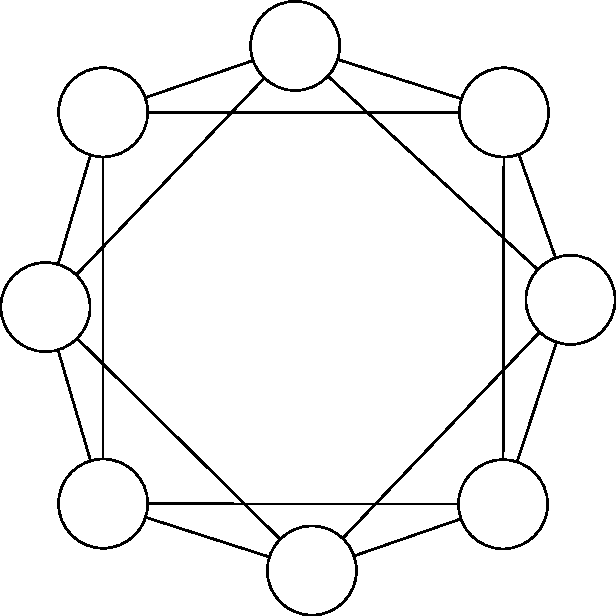
\includegraphics[scale=0.6]{images/dRegular.pdf}
	\caption{$n = 8, d = 4$}
\end{subfigure}
\begin{subfigure}[b]{0.4\textwidth}
	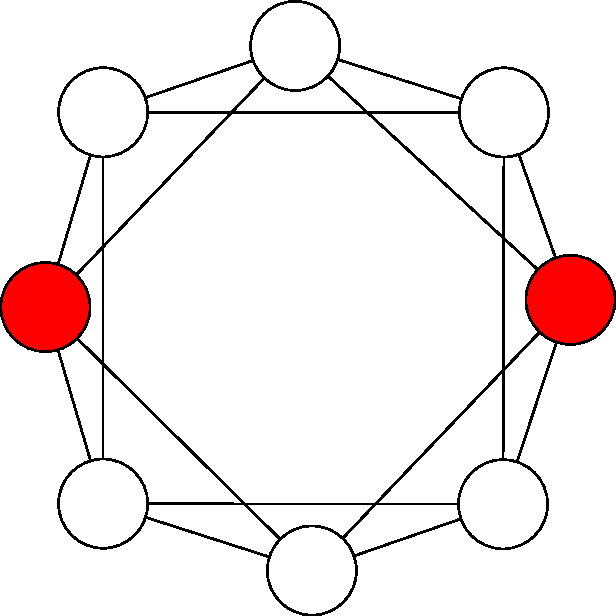
\includegraphics[scale=0.6]{images/dRegularSol.pdf}
	\caption{$\lceil\frac{8}{4}\rceil = 2$}
\end{subfigure}
\end{figure}

Esto vale, ya que al ser un grafo $d$-regular al tomar un nodo ya logro alcanzar $d$ nodos, con lo cual alcanza con tomar $\frac{n}{d}$ nodos de forma correcta, podria llegar a conseguir el CIDM.

Tener la cantidad de nodos nos permite hacer un análisis sobre el tamaño de las soluciones, permitiéndonos tener una mejor perspectiva a la hora de elegir la mejor configuración. Al igual que con los aleatorios, estos grafos poseen dos variable, las cuales son:

\begin{itemize}
	\item La cantidad de nodos
	\item El grado de los nodos (la variable $d$)
\end{itemize}
	
Se siguió una metodología similar que en el caso aleatorio, es decir, para cada $n$ se tomaron 3 valores de $d$, que fueron $\frac{n}{4}$, $\frac{n}{2}$ y $\frac{3n}{4}$.

\subsection{Grafos bipartitos completos}

Al igual que en el caso anterior, la principal razón por la cual decidimos probar con esta familia es que podemos determinar el tamaño de la solución de antemano. Como el grafo es bipartito completo, alcanza con tomar todos los nodos de alguno de los dos conjuntos para poder obtener un CIDM, es decir que para todo grafo bipartito completo la solución va a ser el tamaño del conjunto mas pequeño. Las variables involucradas en este caso son:

\begin{itemize}
	\item La cantidad de nodos en la primer componente
	\item La cantidad de nodos en la segunda componente
\end{itemize}

Para la experimentación se vario la cantidad de nodos de la primer componente, y para cada una de ellas se generaron dos grafos bipartitos completos con $\frac{n}{4}$ y $\frac{3n}{4}$.

\subsection{Arboles binarios}

A diferencia de las dos familias anteriores, donde el tamaño de la solución es único, aquí nos encontramos con un caso donde hay mas de una. Si en un árbol tomamos todos los nodos de un nivel, en el próximo no seria necesario tomar ninguno en el próximo, este patrón se repita hasta llegar al ultimo nivel. Dependiendo de la cantidad de niveles, esto nos permite dar una cota inferior para el CIDM, estas son:

\begin{itemize}
	\item Si la cantidad de niveles es par ($log_2(n)\mod 2 = 0$), la cota inferior es $\mathlarger{\mathlarger{‎\sum}}_{i=0}^{\frac{log_2(n)}{2} - 1} 2^{2i}$
		\item Si la cantidad de niveles es impar ($log_2(n)\mod 2 \neq 0$), la cota inferior es $\mathlarger{\mathlarger{‎\sum}}_{i=0}^{\lfloor\frac{log_2(n)}{2}\rfloor - 1} 2^{2i + 1}$
\end{itemize}

Estas cotas son validos debido a la forma que generamos el grafo, este se va armando de a niveles, y no se crea un nuevo nivel hasta que el anterior se encuentre completo. En el caso que se tenga un Arbol donde existen niveles incompletos, la cota no vale.

Para todo árbol sabemos que la cantidad de conexiones es igual a la cantidad de nodos menos uno, es por esto que para la experimentación se vario únicamente la cantidad de nodos.

\subsection{Cliques}

Al igual que los casos anteriores, se probo también con cliques ya que para cualquier grafo de esta familia sabemos el tamaño de la solución. Para cualquier clique alcanza con tomar un nodo para poder obtener un CIDM, ya que desde esto nodo puedo alcanzar el resto de los nodos del grafo. La idea detrás de experimentar con esta familia es probar la eficiencia de los algoritmos, ya que los mismos deberían poder resolver estos grafos de manera veloz y eficiente.

Al igual que con los arboles binarios, para generar estos grafos solo entra en juego una única variable, y es la cantidad de nodos en el mismo. Al ser una clique, la cantidad de conexiones es siempre $\frac{n(n-1)}{2}$.

\subsection{Grafos unión de componentes conexas}

Por ultimo se decidió probar con un grafo formado por varias componente conexas, unidas por puentes. Cada una de las componentes conexas es un $C_i$, para generar estos grafos se crean sucesivos $C_i$, tomando inicialmente $i = 1$ y aumentando la cantidad de nodos siempre y cuando la cantidad total de nodos los permita. Una vez que las tenemos generadas, se la comienza a unir de manera sucesiva, es decir, se une $C_1$ con $C_2$, $C_2$ con $C_3$, así hasta llegar al ultimo camino generado. La motivación para probar esta familia es poder analizar el impacto que puede llegar a tener la resolución de cada una de las componentes, teniendo en cuenta la presencia de ejes puentes, los cuales pueden afectar el tiempo que toma resolver el grafo.

Esta familia se reservo para ser utilizada como \texttt{test set} al momento de elegir los parámetros óptimos para GRASP. El resto de las familias las utilizaremos como \texttt{training set}.

\subsection{Metodología}

Para hacer el análisis, se hizo variar el valor de $n$ entre 10 y 120. Si el generador para alguna de las familias recibe un segundo parámetro, los utilizados son los mencionados en la sección de cada familia. Para cada valor de $n$ se corrió el algoritmo 100 veces y se tomo el promedio del tiempo.
\newpage

\section{Algoritmo Exacto}

\subsection{Notacion}

Sea $\gamma(G)$ el numero de vertices en el conjunto CIDM.

\subsection{Cotas Superiores e Inferiores}

El problema de
\newpage
%\subsection{Experimentacion}

Para la experimentacion de backtracking se tomo de 6 a 40 nodos, y para cada familia de grafos se tomaron diferentes parametros para la misma cantidad de nodos. Los resultados fueron los siguientes:\\

\begin{figure}[ht]
\centering
	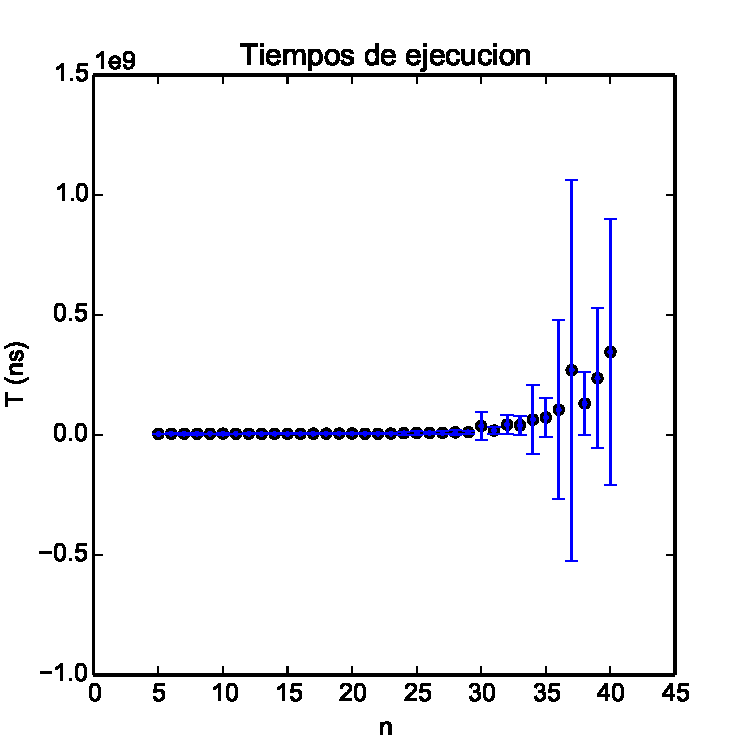
\includegraphics[scale=0.45]{images/graph_ej1/output_backtracking_1_n2}
	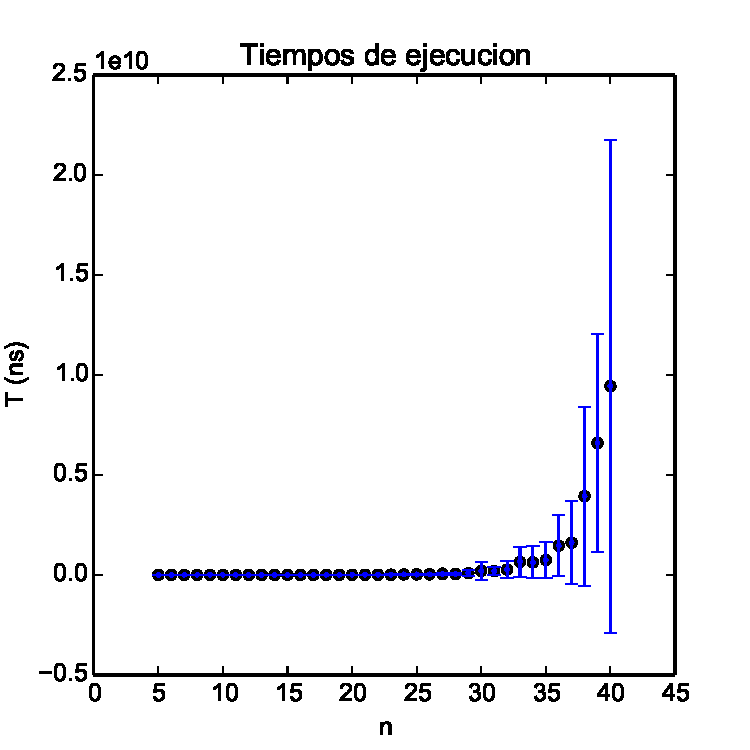
\includegraphics[scale=0.45]{images/graph_ej1/output_backtracking_1_n}
	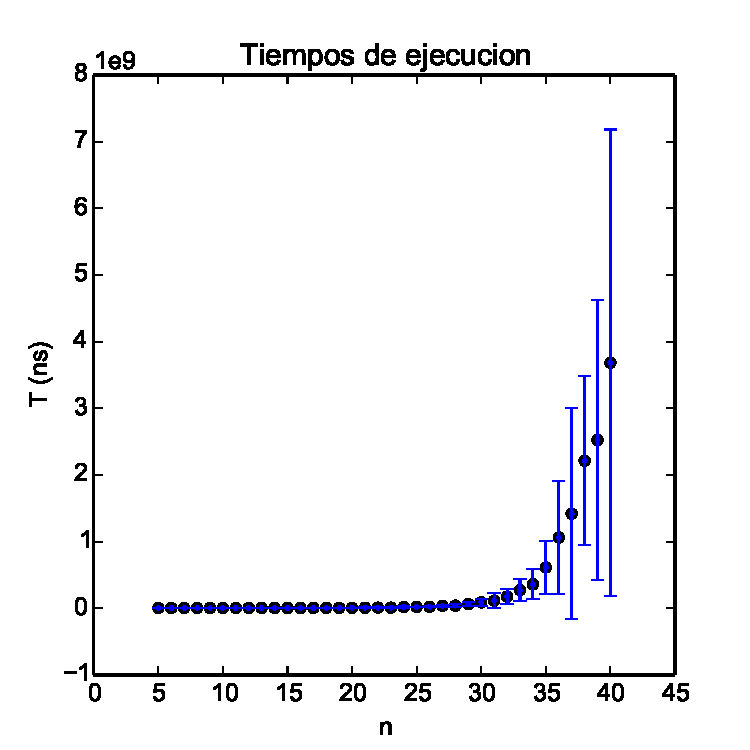
\includegraphics[scale=0.45]{images/graph_ej1/output_backtracking_1_2n}
\end{figure}
\newpage

\section{Heurística Constructiva Golosa}

\subsection{Algoritmos}

Dado que el problema de buscar el CIDM es NP-Hard, para este algoritmo resolveremos el problema por medio de una heurística golosa. La idea básicamente fue ir seleccionando nodos bajo algún criterio, agregándolos al conjunto solución y descartando todos los otros nodos que romperían la independencia de la potencial solución condicional al nodo agregado. Al quedarnos sin nodos para elegir, finalmente tendríamos un conjunto independiente y dominante válido. Dado que la heurística no siempre es optima, muchas veces sucederá que este conjunto que encontraremos no sera el mínimo. Este procedimiento se puede ver en el siguiente pseudocódigo: Para elegir que nodo seleccionar dado los nodos disponibles, utilizaremos la selección por \texttt{grado} y por \texttt{scoring}, que explicaremos a continuación.


\subsubsection{Por grado}

\subsubsection*{Criterio}

Al principio decidimos implementar este criterio de selección de nodos utilizando un heap, ordenando los nodos por su grado. Esto se puede hacer facilmente con el algoritmo de Floyd en Luego, desencolamos del heap y vamos actualizando los flags de cada nodo a medida que son alcanzables. El algoritmo tiene \order{n \times log(n) + m}.

\subsubsection*{Pseudocodigo}

\begin{algorithmic}
\Procedure{greedyHeapConstructive}{G}

\State{nodeHeap $\gets$ buildHeap(G.V)}

\While{!nodeHeap.isEmpty()}
	\State{node $\gets$ nodeHeap.pop()}
	\If{node.reachable == true}
		\State{continue}
	\EndIf
	\State{node.added = true}
	
	\ForAll{$adj \in node.adj$}
		\State{adj.reachable $\gets$ true}
	\EndFor
\EndWhile
\EndProcedure
\end{algorithmic}

\subsubsection{Scoring}

\subsubsection*{Criterio}

Aunque este método con el heap es rápido, en realidad podemos mejorar la forma en la que seleccionamos los vértices. Este método consiste en tomar el número de nodos adyacentes efectivos (score) a los que cada nodo puede acceder. Definimos a un nodo adyacente efectivo como un nodo que es adyacente y a su vez no puede ser accedido por otros nodos que ya pertenecen a la solución parcial en construcción. De esta forma, este criterio también nos garantiza la independencia del conjunto, dado que si tomamos dos nodos de la solución, por construcción no pueden ser adyacentes.

Cada nodo va a tener como atributos su score, un flag que indica si ha sido agregado y otro que indica si es alcanzable por el cubrimiento parcial actual.

El algoritmo va a iterar un arreglo de nodos $n^2$ veces. Cada vez que busquemos un nodo para agregar al conjunto, los iteraremos todos para buscar el de máximo score. Al identificarlo, actualizaremos los scores de los nodos adyacentes a los adyacentes del mismo. A priori parece que la complejidad de este nuevo algoritmo se podría mejorar de forma significativa utilizando algún otro tipo de estructura de datos.

\subsubsection*{Pseudocodigo}

\begin{algorithmic}
\Procedure{greedyConstructive}{G}

\For{i = 0 to i $<$ G.size() }

	\State{greatest $\gets$ 0}
	\State{score $\gets$ 0}
	\State{flag $\gets$ false}

	\For{j = 0 to j $<$ G.size() }
		\If{graph[j] == true}
			\State{continue}
		\EndIf
		\If{graph[j].score $\geq$ score}
			\State{greatest $\gets$ j}
			\State{score $\gets$ graph[j].score}
			\State{flag $\gets$ true}
		\EndIf
	\EndFor

	\If{!flag} \State{break} \EndIf
	
	\State{graph[greatest].added $\gets$ true}
	\State{graph[greatest].reachable $\gets$ true}
	
	\ForAll{$adjNode \in graph[greatest].adj$}
		\State{adjNode.reachable $\gets$ true}
		\ForAll{$adjToAdj \in adjNode.adj$}
			\State{adjToAdj.score--}
		\EndFor
	\EndFor
	
\EndFor
\EndProcedure
\end{algorithmic}

\subsection{Complejidad}

El primer algoritmo resuelve el problema en \order{n \times log(n) + m} simplemente ignorando la actualización de los scores, desencolando de un heap $n$ veces. Sin embargo, este criterio es a simple vista inferior que el de actualización de scores. Aquí hay un tradeoff entre hacer la mejor elección y la complejidad temporal del algoritmo.

El algoritmo basado en el score recorre arreglo $n$ veces. A su vez, buscar los adyacentes de los adyacentes se hace $m$ veces en total. Luego actualizamos en total el score de $m$ nodos. Por lo tanto, el algoritmo tiene orden \order{n^2 + 2 \times m}, es decir \order{n^2}.

Notar que la forma en que buscamos el máximo es sumamente ineficiente. Esto se debe a que si utilizamos sort, luego es bastante difícil encontrar el nodo al que le debemos actualizar su respectivo score. A su vez, dado que en cada iteración actualizamos el score, mantener el orden es sumamente costoso. Es muy posible que exista una estructura de datos mucho más eficiente para resolver este problema (una especie de heap dinámico), aunque para este trabajo practico nos conformaremos con el algoritmo en \order{n^2}.

\subsection{Efectividad de la heurística}

Nuestra heurística no siempre devuelve la solución optima. Considerar los siguientes ejemplos:

\begin{figure}[ht]
\centering
\begin{subfigure}[b]{0.4\textwidth}
	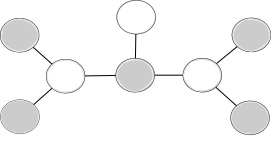
\includegraphics[scale=0.6]{images/greedy_fail.png}
	\caption{Greedy (5 nodos)}
\end{subfigure}
\begin{subfigure}[b]{0.4\textwidth}
	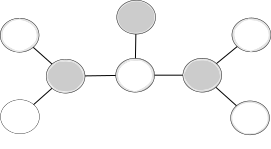
\includegraphics[scale=0.6]{images/greedy_best.png}
	\caption{Óptimo (3 nodos)}
\end{subfigure}

\begin{subfigure}[b]{0.4\textwidth}
	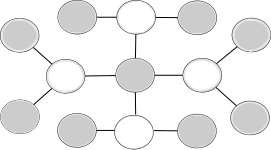
\includegraphics[scale=0.6]{images/greedy_fail2.png}
	\caption{Greedy (9 nodos)}
\end{subfigure}
\begin{subfigure}[b]{0.4\textwidth}
	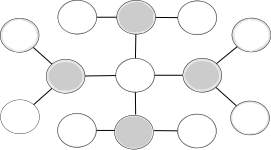
\includegraphics[scale=0.6]{images/greedy_best2.png}
	\caption{Óptimo (4 nodos)}
\end{subfigure}
\caption{Ejemplos de nuestra heurística comparado con el óptimo.}
\end{figure}

El peor caso es claramente el de la figura (c) y (d). Tenemos un nodo $v$ (el nodo central) de grado $d(v) = 4$, con sus nodos adyacentes de grado $d(u) = 3$. Si tenemos $c$ componentes conexas de ese tipo, utilizaremos $c \times (2 \times 4 + 1)$ nodos, cuando en realidad el optimo tiene $c \times 4$ nodos.




\newpage
\subsection{Experimentación}

Para la experimentación se siguió con la metodología indicada anteriormente. Los resultados fueron los siguientes.

\subsubsection{Heurística Constructiva Golosa por Grado}

Los resultados temporales obtenidos fueron los siguientes:

\begin{figure}[H]
\centering

\begin{subfigure}[h]{0.4\textwidth}
	\includegraphics[scale=0.6]{graph/{output_greedy_1_1_n.csvTime}.pdf}
	\begin{center}
	Grafos Aleatorios ($m = n$)
	\end{center}
\end{subfigure}
\begin{subfigure}[h]{0.4\textwidth}
	\includegraphics[scale=0.6]{graph/{output_greedy_1_1_2n.csvTime}.pdf}
	\begin{center}
	Grafos Aleatorios ($m = 2n$)
	\end{center}
\end{subfigure}

\begin{subfigure}[h]{0.4\textwidth}
	\includegraphics[scale=0.6]{graph/{output_greedy_1_1_n2.csvTime}.pdf}
	\begin{center}
	Grafos Aleatorios ($m = \frac{n}{2}$)
	\end{center}
\end{subfigure}
\begin{subfigure}[h]{0.4\textwidth}
	\includegraphics[scale=0.6]{graph/{output_greedy_1_3_n4.csvTime}.pdf}
	\begin{center}
	Grafos Bipartitos ($\frac{n}{4}$ nodos en la segunda componente)
	\end{center}
\end{subfigure}
\end{figure}

\begin{figure}[H]
\centering

\begin{subfigure}[h]{0.4\textwidth}
	\includegraphics[scale=0.6]{graph/{output_greedy_1_3_3n4.csvTime}.pdf}
	\begin{center}
	Grafos Bipartitos ($\frac{3n}{4}$ nodos en la segunda componente)
	\end{center}
\end{subfigure}
\begin{subfigure}[h]{0.4\textwidth}
	\includegraphics[scale=0.6]{graph/{output_greedy_1_2_n4.csvTime}.pdf}
	\begin{center}
	Grafos $d$-regulares ($d = \frac{n}{4}$)
	\end{center}
\end{subfigure}

\begin{subfigure}[h]{0.4\textwidth}
	\includegraphics[scale=0.6]{graph/{output_greedy_1_2_n2.csvTime}.pdf}
	\begin{center}
	Grafos $d$-regulares ($m = \frac{n}{2}$)
	\end{center}
\end{subfigure}
\begin{subfigure}[h]{0.4\textwidth}
	\includegraphics[scale=0.6]{graph/{output_greedy_1_2_3n4.csvTime}.pdf}
	\begin{center}
	Grafos $d$-regulares ($m = \frac{3n}{4}$)
	\end{center}
\end{subfigure}
\end{figure}

\newpage
\begin{figure}
\centering

\begin{subfigure}[h]{0.4\textwidth}
	\includegraphics[scale=0.6]{graph/{output_greedy_1_4_arbol.csvTime}.pdf}
	\begin{center}
	Arboles Binarios
	\end{center}
\end{subfigure}
\begin{subfigure}[h]{0.4\textwidth}
	\includegraphics[scale=0.6]{graph/{output_greedy_1_1_clique.csvTime}.pdf}
	\begin{center}
	Clique
	\end{center}
\end{subfigure}
\end{figure}

\newpage
Primero vamos a ver los resultados por cada familia.

\begin{itemize}
	\item Grafos aleatorios: En este caso podemos ver que la cantidad de conexiones entre nodos afecto al tiempo. De todas maneras el impacto no fue tan grande como esperábamos. En el caso $n = 120$ la diferencia entre $m = \frac{n}{4}$ y $m = 2n$ fue, en promedio, de 218 segundos.
	\item Grafos bipartitos: En este caso nos sorprendió el tiempo que tardo el algoritmo en poder encontrar solución. Consideramos que esto se debe a que en un grafo bipartito completo existen solo dos posibles cubrimientos. Otro detalle a destacar fue el aumento en tiempo que hubo mientras mas equilibradas se encontraban las dos componentes del grafo, con $\frac{3n}{4}$ nodos en la segunda componente se convergió a un resultado en un tiempo mucho mayor.
	\item Grafos $d$-regulares: Aquí a diferencia de los grafos aleatorios, al haber una diferencia mas marcada entre la cantidad de conexiones se puede ver en el gráfico que la diferencia entre $d = \frac{n}{4}$ y $d = \frac{3n}{4}$ es muy marcada, la misma siendo de varios minutos.
	\item Arboles binarios: En este caso, podemos observar que el tiempo de ejecución se comporta de forma creciente sobre $n$. Hay dos outliers que arruinan la escala del gráfico, pero podemos observar que la tendencia es como mínimo lineal. Esto tiene sentido dado que estamos agregando solo un nodo y una arista por cada aumento en $n$.
	\item Cliques: Las cliques se comportaron de manera esperada, al ser un caso fácil de resolver el algoritmo no tuvo mayores dificultades.
\end{itemize}

Para el análisis del tamaño de la solución, vamos a ver los resultados por cada familia. En el caso de los aleatorios, los resultados para estas configuraciones fueron los siguientes:

\begin{table}[H]
\centering
\label{my-label}
\begin{tabular}{|l|lll|}
\hline
        & \multicolumn{1}{l|}{m = n/2} & \multicolumn{1}{l|}{m = n} & m = 2n \\ \hline
n = 40  & 26                           & 21                         & 12     \\ \cline{1-1}
n = 60  & 38                           & 27                         & 16     \\ \cline{1-1}
n = 80  & 49                           & 33                         & 21     \\ \cline{1-1}
n = 100 & 59                           & 42                         & 24     \\ \cline{1-1}
n = 120 & 74                           & 55                         & 28     \\ \hline
\end{tabular}
\caption{Grafos aleatorios. Los números en la tabla muestran la cantidad de vértices en el conjunto dominante independiente final.}
\end{table}

Los tamaños de resultados se comportaron de manera esperada, es decir, a medida que aumento la cantidad de aristas se redujo el cardinal del conjunto solución.

Para los Grafos Bipartitos, los $d$-regulares y las cliques, el algoritmo encontró la solución optima en todos los casos. Respecto a los arboles, la solución del algoritmo siempre respeto la cota y el resultado fue el menor posible.

\subsubsection{Heurística Constructiva Golosa por Scoring}

Los resultados temporales obtenidos fueron los siguientes:

\begin{figure}[H]
\centering

\begin{subfigure}[h]{0.4\textwidth}
	\includegraphics[scale=0.6]{graph/{output_greedy_2_1_n.csvTime}.pdf}
	\begin{center}
	Grafos Aleatorios ($m = n$)
	\end{center}
\end{subfigure}
\begin{subfigure}[h]{0.4\textwidth}
	\includegraphics[scale=0.6]{graph/{output_greedy_2_1_2n.csvTime}.pdf}
	\begin{center}
	Grafos Aleatorios ($m = 2n$)
	\end{center}
\end{subfigure}

\begin{subfigure}[h]{0.4\textwidth}
	\includegraphics[scale=0.6]{graph/{output_greedy_2_1_n2.csvTime}.pdf}
	\begin{center}
	Grafos Aleatorios ($m = \frac{n}{2}$)
	\end{center}
\end{subfigure}
\begin{subfigure}[h]{0.4\textwidth}
	\includegraphics[scale=0.6]{graph/{output_greedy_2_3_n4.csvTime}.pdf}
	\begin{center}
	Grafos Bipartitos ($\frac{n}{4}$ nodos en la segunda componente)
	\end{center}
\end{subfigure}
\end{figure}

\begin{figure}[H]
\centering

\begin{subfigure}[h]{0.4\textwidth}
	\includegraphics[scale=0.6]{graph/{output_greedy_2_3_3n4.csvTime}.pdf}
	\begin{center}
	Grafos Bipartitos ($\frac{3n}{4}$ nodos en la segunda componente)
	\end{center}
\end{subfigure}
\begin{subfigure}[h]{0.4\textwidth}
	\includegraphics[scale=0.6]{graph/{output_greedy_2_2_n4.csvTime}.pdf}
	\begin{center}
	Grafos $d$-regulares ($d = \frac{n}{4}$)
	\end{center}
\end{subfigure}

\begin{subfigure}[h]{0.4\textwidth}
	\includegraphics[scale=0.6]{graph/{output_greedy_2_2_n2.csvTime}.pdf}
	\begin{center}
	Grafos $d$-regulares ($m = \frac{n}{2}$)
	\end{center}
\end{subfigure}
\begin{subfigure}[h]{0.4\textwidth}
	\includegraphics[scale=0.6]{graph/{output_greedy_2_2_3n4.csvTime}.pdf}
	\begin{center}
	Grafos $d$-regulares ($m = \frac{3n}{4}$)
	\end{center}
\end{subfigure}
\end{figure}

\newpage
\begin{figure}
\centering

\begin{subfigure}[b]{0.4\textwidth}
	\includegraphics[scale=0.6]{graph/{output_greedy_2_4_arbol.csvTime}.pdf}
	\begin{center}
	Arboles Binarios
	\end{center}
\end{subfigure}
\begin{subfigure}[b]{0.4\textwidth}
	\includegraphics[scale=0.6]{graph/{output_greedy_2_1_clique.csvTime}.pdf}
	\begin{center}
	Clique
	\end{center}
\end{subfigure}
\end{figure}

\newpage
Los resultados obtenidos por familia no difirieron en gran medida respecto a lo obtenido con la Heurística Constructiva Golosa por Grado, con lo cual respecto al tiempo se derivan las misma conclusiones de antes.

Para el análisis del tamaño de la solución, vamos a ver los resultados por cada familia. En el caso de los aleatorios, los resultados para estas configuraciones fueron los siguiente:

\begin{table}[H]
\centering
\label{my-label}
\begin{tabular}{|l|lll|}
\hline
        & \multicolumn{1}{l|}{m = n/2} & \multicolumn{1}{l|}{m = n} & m = 2n \\ \hline
n = 40  & 32                           & 26                         & 16     \\ \cline{1-1}
n = 60  & 43                           & 33                         & 16     \\ \cline{1-1}
n = 80  & 56                           & 44                         & 30     \\ \cline{1-1}
n = 100 & 67                           & 56                         & 40     \\ \cline{1-1}
n = 120 & 74                           & 66                         & 46     \\ \hline
\end{tabular}
\caption{Grafos aleatorios. Los números en la tabla muestran la cantidad de vértices en el conjunto dominante independiente final.}
\end{table}

Aquí es donde la diferencia es mas marcada, para los mismos casos, la Heurística por Scoring dio resultados significativamente peores en el caso aleatorio. Esto también se vio reflejado en las otras familias también, particularmente en el caso de los bipartitos donde siempre se priorizo la solución mas grande.

\subsubsection{Conclusión}

En lo que respecta al tiempo de ejecución, las heurísticas no se comportaron de manera muy diferente, el tiempo fue similar. Sin embargo, recordemos que la heurística por grado utiliza un heap como estructura de datos auxiliar, por lo que para tamaños de $n$ más grandes la diferencia se notaria más. El lugar donde la diferencia fue significativa fue en el tamaño de las soluciones obtenidas, donde en prácticamente todos los casos la Heurística Constructiva por Grado dio mejor resultado, con lo cual consideramos que de las golosas, es mejor la selección por grado que por scoring.
\newpage

\section{Heurística de Búsqueda Local}

\subsection{Algoritmo}

Antes de explicar nuestro algoritmo, comenzemos definiendo que es una heurística de búsqueda local. Para cada solución factible $s \in S$, se define $N(s)$ como el conjunto de soluciones vecinas de $s$. Un procedimiento de búsqueda local toma una solución inicial $s$ e iterativamente la mejora reemplazándola por otra solución mejor del conjunto $N(s)$, hasta llegar a un optimo local. El algoritmo se puede ver con el siguiente pseudocodigo:

\begin{algorithmic}
\Procedure{localSearch}{G}
\State{s $\gets$ getInitialSolution(G)}
\State{localSolution $\gets$ true}
\While{localSolution}
	\State{$localSolution \gets false$}
	\ForAll{$\hat{s} \in N(s)$}
		\If{$|\hat{s}| < |s|$}
			\State{$s \gets \hat{s}$}
			\State{$localSolution \gets true$}
			\State{break}
		\EndIf
	\EndFor
\EndWhile
\EndProcedure
\end{algorithmic}

\hspace{1px}

En primer lugar hay que pensar que algoritmo utilizar en la función $getInitialSolution(G)$. Para esto, utilizamos cualquiera de las heurísticas constructivas golosas del paso anterior.

Luego, debemos identificar como construiremos las diferentes $s \in N(s)$, es decir, como construiremos la función que nos devuelve los vecinos de una solución parcial $N(S)$.

\subsection{Vecindades}

Para este algoritmo, utilizaremos los siguientes dos criterios para definir la vecindad de una solución $s$:

\begin{enumerate}
\item \underline{Primera vecindad:}
Para la primera vecindad simplemente tomamos un vértice que actualmente no pertenece a la solución local. Luego, quitamos todos sus vértices adyacentes y verificamos si tenemos una solución con menor cardinal.
\item \underline{Segunda vecindad:}
Para este criterio, lo que hacemos es buscar dos nodos que no pertenecen a la solución local. Los agregamos, quitamos sus nodos adyacentes, y verificamos si el nuevo conjunto es un cubrimiento de menor cardinal.
\end{enumerate}

\subsection{Complejidad}

\subsubsection{Primera vecindad}

En una iteración, el primer algoritmo de vecindad agrega un nodo y luego quita sus adyacentes. Luego verifica que los adyacentes de estos vértices que hemos quitado son alcanzables. Por lo tanto, en el peor caso una iteración tiene orden \order{n \times \Delta(G)^3}. Esto se debe a que se debe verificar que todos los nodos adyacentes a los que saque son adyacentes a algún otro nodo del conjunto en \order{\Delta(G)} para cada nodo adyacente ($\Delta(G)$) a los adyacentes que pude quitar ($\Delta(G)$). Si el nuevo conjunto de nodos no es un CIDM, simplemente restauramos el grafo en \order{\Delta(G)}.

\subsubsection{Segunda vecindad}

En el segundo caso, probamos agregando todos los pares de nodos a la solución actual, quitando sus nodos adyacentes y verificando si luego es una solución. Para ello, simplemente repetimos el procedimiento de la primera vecindad.

Este procedimiento lo repetimos para todo par de $v \not\in S$. Podemos acotar esto de forma grotesca por $\binom{n}{2}$. Por lo tanto la complejidad total de una iteración es de \order{\binom{n}{2} \times \Delta(G)^3}.

\newpage
%\subsection{Experimentación}

Para la experimentación se siguió con la metodología indicada anteriormente. Los resultados fueron los siguientes.

\subsubsection{Heurística Constructiva Golosa por Scoring con Búsqueda Local por primer Vecinidad}

Los resultados temporales obtenidos fueron los siguientes:

\begin{figure}[H]
\centering

\begin{subfigure}[h]{0.4\textwidth}
	\includegraphics[scale=0.5]{graph/{output_local_1_1_n.csvTime}.pdf}
	\begin{center}
	Grafos Aleatorios ($m = n$)
	\end{center}
\end{subfigure}
\begin{subfigure}[h]{0.4\textwidth}
	\includegraphics[scale=0.5]{graph/{output_local_1_1_2n.csvTime}.pdf}
	\begin{center}
	Grafos Aleatorios ($m = 2n$)
	\end{center}
\end{subfigure}

\begin{subfigure}[h]{0.4\textwidth}
	\includegraphics[scale=0.5]{graph/{output_local_1_1_n2.csvTime}.pdf}
	\begin{center}
	Grafos Aleatorios ($m = \frac{n}{2}$)
	\end{center}
\end{subfigure}
\begin{subfigure}[h]{0.4\textwidth}
	\includegraphics[scale=0.5]{graph/{output_local_1_3_n4.csvTime}.pdf}
	\begin{center}
	Grafos Bipartitos ($\frac{n}{4}$ nodos en la segunda componente)
	\end{center}
\end{subfigure}
\end{figure}

\begin{figure}[H]
\centering

\begin{subfigure}[h]{0.4\textwidth}
	\includegraphics[scale=0.5]{graph/{output_local_1_3_3n4.csvTime}.pdf}
	\begin{center}
	Grafos Bipartitos ($\frac{3n}{4}$ nodos en la segunda componente)
	\end{center}
\end{subfigure}
\begin{subfigure}[h]{0.4\textwidth}
	\includegraphics[scale=0.5]{graph/{output_local_1_2_n4.csvTime}.pdf}
	\begin{center}
	Grafos $d$-regulares ($d = \frac{n}{4}$)
	\end{center}
\end{subfigure}

\begin{subfigure}[h]{0.4\textwidth}
	\includegraphics[scale=0.5]{graph/{output_local_1_2_n2.csvTime}.pdf}
	\begin{center}
	Grafos $d$-regulares ($m = \frac{n}{2}$)
	\end{center}
\end{subfigure}
\begin{subfigure}[h]{0.4\textwidth}
	\includegraphics[scale=0.5]{graph/{output_local_1_2_3n4.csvTime}.pdf}
	\begin{center}
	Grafos $d$-regulares ($m = \frac{3n}{4}$)
	\end{center}
\end{subfigure}
\end{figure}

\begin{figure}[H]
\centering

\begin{subfigure}[h]{0.4\textwidth}
	\includegraphics[scale=0.5]{graph/{output_local_1_4_arbol.csvTime}.pdf}
	\begin{center}
	Arboles Binarios
	\end{center}
\end{subfigure}
\begin{subfigure}[h]{0.4\textwidth}
	\includegraphics[scale=0.5]{graph/{output_local_1_1_clique.csvTime}.pdf}
	\begin{center}
	Clique
	\end{center}
\end{subfigure}
\end{figure}

Para el análisis del tamaño de la solución, vamos a ver los resultados por cada familia. En el caso de los aleatorios, los resultados para estas configuraciones fueron los siguientes:

\begin{table}[H]
\centering
\label{my-label}
\begin{tabular}{|l|lll|}
\hline
        & \multicolumn{1}{l|}{m = n/2} & \multicolumn{1}{l|}{m = n} & m = 2n \\ \hline
n = 40  & 26                           & 21                         & 12     \\ \cline{1-1}
n = 60  & 38                           & 27                         & 16     \\ \cline{1-1}
n = 80  & 49                           & 33                         & 21     \\ \cline{1-1}
n = 100 & 59                           & 42                         & 24     \\ \cline{1-1}
n = 120 & 74                           & 55                         & 28     \\ \hline
\end{tabular}
\caption{Grafos aleatorios. Los números en la tabla muestran la cantidad de vértices en el conjunto dominante independiente final.}
\end{table}

Los tamaños obtenidos en el caso aleatorio son los mismos que los obtenidos mediante la solución inicial, es decir, la búsqueda local no mejoro ninguna de las soluciones.

Para los Grafos Bipartitos, los $d$-regulares y las cliques, el algoritmo encontró la solución optima en todos los casos. Respecto a los arboles, la solución del algoritmo siempre respeto la cota y el resultado fue el menor posible.

\subsubsection{Heurística Constructiva Golosa por Scoring con Búsqueda Local por segunda Vecinidad}

Los resultados temporales obtenidos fueron los siguientes:

\begin{figure}[H]
\centering

\begin{subfigure}[h]{0.4\textwidth}
	\includegraphics[scale=0.5]{graph/{output_local_2_1_n.csvTime}.pdf}
	\begin{center}
	Grafos Aleatorios ($m = n$)
	\end{center}
\end{subfigure}
\begin{subfigure}[h]{0.4\textwidth}
	\includegraphics[scale=0.5]{graph/{output_local_2_1_2n.csvTime}.pdf}
	\begin{center}
	Grafos Aleatorios ($m = 2n$)
	\end{center}
\end{subfigure}

\begin{subfigure}[h]{0.4\textwidth}
	\includegraphics[scale=0.5]{graph/{output_local_2_1_n2.csvTime}.pdf}
	\begin{center}
	Grafos Aleatorios ($m = \frac{n}{2}$)
	\end{center}
\end{subfigure}
\begin{subfigure}[h]{0.4\textwidth}
	\includegraphics[scale=0.5]{graph/{output_local_2_3_n4.csvTime}.pdf}
	\begin{center}
	Grafos Bipartitos ($\frac{n}{4}$ nodos en la segunda componente)
	\end{center}
\end{subfigure}
\end{figure}

\begin{figure}[H]
\centering

\begin{subfigure}[h]{0.4\textwidth}
	\includegraphics[scale=0.5]{graph/{output_local_2_3_3n4.csvTime}.pdf}
	\begin{center}
	Grafos Bipartitos ($\frac{3n}{4}$ nodos en la segunda componente)
	\end{center}
\end{subfigure}
\begin{subfigure}[h]{0.4\textwidth}
	\includegraphics[scale=0.5]{graph/{output_local_2_2_n4.csvTime}.pdf}
	\begin{center}
	Grafos $d$-regulares ($d = \frac{n}{4}$)
	\end{center}
\end{subfigure}

\begin{subfigure}[h]{0.4\textwidth}
	\includegraphics[scale=0.5]{graph/{output_local_2_2_n2.csvTime}.pdf}
	\begin{center}
	Grafos $d$-regulares ($m = \frac{n}{2}$)
	\end{center}
\end{subfigure}
\begin{subfigure}[h]{0.4\textwidth}
	\includegraphics[scale=0.5]{graph/{output_local_2_2_3n4.csvTime}.pdf}
	\begin{center}
	Grafos $d$-regulares ($m = \frac{3n}{4}$)
	\end{center}
\end{subfigure}
\end{figure}

\begin{figure}[H]
\centering

\begin{subfigure}[h]{0.4\textwidth}
	\includegraphics[scale=0.5]{graph/{output_local_2_4_arbol.csvTime}.pdf}
	\begin{center}
	Arboles Binarios
	\end{center}
\end{subfigure}
\begin{subfigure}[h]{0.4\textwidth}
	\includegraphics[scale=0.5]{graph/{output_local_2_1_clique.csvTime}.pdf}
	\begin{center}
	Clique
	\end{center}
\end{subfigure}
\end{figure}

Para el análisis del tamaño de la solución, vamos a ver los resultados por cada familia. En el caso de los aleatorios, los resultados para estas configuraciones fueron los siguientes:

\begin{table}[H]
\centering
\label{my-label}
\begin{tabular}{|l|lll|}
\hline
        & \multicolumn{1}{l|}{m = n/2} & \multicolumn{1}{l|}{m = n} & m = 2n \\ \hline
n = 40  & 26                           & 21                         & 12     \\ \cline{1-1}
n = 60  & 38                           & 27                         & 16     \\ \cline{1-1}
n = 80  & 49                           & 33                         & 21     \\ \cline{1-1}
n = 100 & 59                           & 42                         & 24     \\ \cline{1-1}
n = 120 & 74                           & 55                         & 28     \\ \hline
\end{tabular}
\caption{Grafos aleatorios. Los números en la tabla muestran la cantidad de vértices en el conjunto dominante independiente final.}
\end{table}

Al igual que con la primer vecinidad, no se pudo mejorar la solución original. Respecto al resto de las familias, las soluciones fueron optimas y los resultados fueron cercanos a las cotas de cada familia.

\subsubsection{Heurística Constructiva Golosa por Grado con Búsqueda Local por primer Vecinidad}

Los resultados temporales obtenidos fueron los siguientes:

\begin{figure}[H]
\centering

\begin{subfigure}[h]{0.4\textwidth}
	\includegraphics[scale=0.5]{graph/{output_local_3_1_n.csvTime}.pdf}
	\begin{center}
	Grafos Aleatorios ($m = n$)
	\end{center}
\end{subfigure}
\begin{subfigure}[h]{0.4\textwidth}
	\includegraphics[scale=0.5]{graph/{output_local_3_1_2n.csvTime}.pdf}
	\begin{center}
	Grafos Aleatorios ($m = 2n$)
	\end{center}
\end{subfigure}

\begin{subfigure}[h]{0.4\textwidth}
	\includegraphics[scale=0.5]{graph/{output_local_3_1_n2.csvTime}.pdf}
	\begin{center}
	Grafos Aleatorios ($m = \frac{n}{2}$)
	\end{center}
\end{subfigure}
\begin{subfigure}[h]{0.4\textwidth}
	\includegraphics[scale=0.5]{graph/{output_local_3_3_n4.csvTime}.pdf}
	\begin{center}
	Grafos Bipartitos ($\frac{n}{4}$ nodos en la segunda componente)
	\end{center}
\end{subfigure}
\end{figure}

\begin{figure}[H]
\centering

\begin{subfigure}[h]{0.4\textwidth}
	\includegraphics[scale=0.5]{graph/{output_local_3_3_3n4.csvTime}.pdf}
	\begin{center}
	Grafos Bipartitos ($\frac{3n}{4}$ nodos en la segunda componente)
	\end{center}
\end{subfigure}
\begin{subfigure}[h]{0.4\textwidth}
	\includegraphics[scale=0.5]{graph/{output_local_3_2_n4.csvTime}.pdf}
	\begin{center}
	Grafos $d$-regulares ($d = \frac{n}{4}$)
	\end{center}
\end{subfigure}

\begin{subfigure}[h]{0.4\textwidth}
	\includegraphics[scale=0.5]{graph/{output_local_3_2_n2.csvTime}.pdf}
	\begin{center}
	Grafos $d$-regulares ($m = \frac{n}{2}$)
	\end{center}
\end{subfigure}
\begin{subfigure}[h]{0.4\textwidth}
	\includegraphics[scale=0.5]{graph/{output_local_3_2_3n4.csvTime}.pdf}
	\begin{center}
	Grafos $d$-regulares ($m = \frac{3n}{4}$)
	\end{center}
\end{subfigure}
\end{figure}

\begin{figure}[H]
\centering

\begin{subfigure}[h]{0.4\textwidth}
	\includegraphics[scale=0.5]{graph/{output_local_3_4_arbol.csvTime}.pdf}
	\begin{center}
	Arboles Binarios
	\end{center}
\end{subfigure}
\begin{subfigure}[h]{0.4\textwidth}
	\includegraphics[scale=0.5]{graph/{output_local_3_1_clique.csvTime}.pdf}
	\begin{center}
	Clique
	\end{center}
\end{subfigure}
\end{figure}

Para el análisis del tamaño de la solución, vamos a ver los resultados por cada familia. En el caso de los aleatorios, los resultados para estas configuraciones fueron los siguientes:

\begin{table}[H]
\centering
\label{my-label}
\begin{tabular}{|l|lll|}
\hline
        & \multicolumn{1}{l|}{m = n/2} & \multicolumn{1}{l|}{m = n} & m = 2n \\ \hline
n = 40  & 32                           & 26                         & 16     \\ \cline{1-1}
n = 60  & 43                           & 33                         & 22     \\ \cline{1-1}
n = 80  & 56                           & 44                         & 30     \\ \cline{1-1}
n = 100 & 67                           & 56                         & 40     \\ \cline{1-1}
n = 120 & 74                           & 66                         & 46     \\ \hline
\end{tabular}
\caption{Grafos aleatorios. Los números en la tabla muestran la cantidad de vértices en el conjunto dominante independiente final.}
\end{table}

Al igual que con el primer criterio de vecinidad, en el caso de los aleatorios la solución no mejoro, se mantuvo en los mismo valores de la original. Sin embargo, este presento mejoras en los Arboles, dando una solución menor.

\subsubsection{Heurística Constructiva Golosa por Grado con Búsqueda Local por segunda Vecinidad}

Los resultados temporales obtenidos fueron los siguientes:

\begin{figure}[H]
\centering

\begin{subfigure}[h]{0.4\textwidth}
	\includegraphics[scale=0.5]{graph/{output_local_4_1_n.csvTime}.pdf}
	\begin{center}
	Grafos Aleatorios ($m = n$)
	\end{center}
\end{subfigure}
\begin{subfigure}[h]{0.4\textwidth}
	\includegraphics[scale=0.5]{graph/{output_local_4_1_2n.csvTime}.pdf}
	\begin{center}
	Grafos Aleatorios ($m = 2n$)
	\end{center}
\end{subfigure}

\begin{subfigure}[h]{0.4\textwidth}
	\includegraphics[scale=0.5]{graph/{output_local_4_1_n2.csvTime}.pdf}
	\begin{center}
	Grafos Aleatorios ($m = \frac{n}{2}$)
	\end{center}
\end{subfigure}
\begin{subfigure}[h]{0.4\textwidth}
	\includegraphics[scale=0.5]{graph/{output_local_4_3_n4.csvTime}.pdf}
	\begin{center}
	Grafos Bipartitos ($\frac{n}{4}$ nodos en la segunda componente)
	\end{center}
\end{subfigure}
\end{figure}

\begin{figure}[H]
\centering

\begin{subfigure}[h]{0.4\textwidth}
	\includegraphics[scale=0.5]{graph/{output_local_4_3_3n4.csvTime}.pdf}
	\begin{center}
	Grafos Bipartitos ($\frac{3n}{4}$ nodos en la segunda componente)
	\end{center}
\end{subfigure}
\begin{subfigure}[h]{0.4\textwidth}
	\includegraphics[scale=0.5]{graph/{output_local_4_2_n4.csvTime}.pdf}
	\begin{center}
	Grafos $d$-regulares ($d = \frac{n}{4}$)
	\end{center}
\end{subfigure}

\begin{subfigure}[h]{0.4\textwidth}
	\includegraphics[scale=0.5]{graph/{output_local_4_2_n2.csvTime}.pdf}
	\begin{center}
	Grafos $d$-regulares ($m = \frac{n}{2}$)
	\end{center}
\end{subfigure}
\begin{subfigure}[h]{0.4\textwidth}
	\includegraphics[scale=0.5]{graph/{output_local_4_2_3n4.csvTime}.pdf}
	\begin{center}
	Grafos $d$-regulares ($m = \frac{3n}{4}$)
	\end{center}
\end{subfigure}
\end{figure}

\begin{figure}[H]
\centering

\begin{subfigure}[h]{0.4\textwidth}
	\includegraphics[scale=0.5]{graph/{output_local_4_4_arbol.csvTime}.pdf}
	\begin{center}
	Arboles Binarios
	\end{center}
\end{subfigure}
\begin{subfigure}[h]{0.4\textwidth}
	\includegraphics[scale=0.5]{graph/{output_local_4_1_clique.csvTime}.pdf}
	\begin{center}
	Clique
	\end{center}
\end{subfigure}
\end{figure}

Para el análisis del tamaño de la solución, vamos a ver los resultados por cada familia. En el caso de los aleatorios, los resultados para estas configuraciones fueron los siguientes:

\begin{table}[H]
\centering
\label{my-label}
\begin{tabular}{|l|lll|}
\hline
        & \multicolumn{1}{l|}{m = n/2} & \multicolumn{1}{l|}{m = n} & m = 2n \\ \hline
n = 40  & 27                           & 20                         & 16     \\ \cline{1-1}
n = 60  & 40                           & 33                         & 22     \\ \cline{1-1}
n = 80  & 52                           & 42                         & 27     \\ \cline{1-1}
n = 100 & 65                           & 51                         & 31     \\ \cline{1-1}
n = 120 & 80                           & 62                         & 40     \\ \hline
\end{tabular}
\caption{Grafos aleatorios. Los números en la tabla muestran la cantidad de vértices en el conjunto dominante independiente final.}
\end{table}

A diferencia de los otros casos, aquí podemos ver como la segunda vecindad mejoro amplimente el resultado anterior, a tal punto que se llego a un mejor resultado que el obtenido con la Heurística Constructiva Golosa por Scoring.

\subsubsection{Conclusión}

Primero vamos a ver los resultados por cada familia.

\begin{itemize}
	\item Grafos Aleatorios: Como era de esperar la cantidad de conexiones volvió a impactar en el tiempo de cada algoritmo. También pudimos apreciar el costo agregado del segundo criterio de vecindad, ya que en los casos donde se lo aplico, los tiempos aumentaron de manera considerable.
	\item Grafos Bipartitos: El tiempo de convergencia al aplicar el segundo criterio de vecindad aumento considerablemente, esto es un detrimento importante, ya que la solución inicial no fue mejorada.
	\item Grafos $d$-regulares: Aquí también los tiempos de ejecucion aumentaron, sin embargo, el aumento no fue tan pronunciado como en las dos familias anteriores.
	\item Arboles binarios: A diferencia de los casos anteriores, los tiempos obtenidos aquí no difieren mucho entre vecinidades. Estas tampoco pudieron lograr una mejora importante respecto a la solucion original.
	\item Cliques: En las cliques sabemos que toda solución puede tener a lo sumo un nodo, con lo cual la misma no puede ser mejorada. Los dos criterios de vecinidad tomaron tiempos similares de ejecucion.
\end{itemize}

La eficiencia del primer criterio de vecinidad fue limitada, si bien el mismo no introducía mucho tiempo extra en la ejecución del algoritmo, no podía mejorar las solución por un margen razonable. Por el otro lado, el segundo criterio de vecinidad logro demostrar su efectividad para poder mejorar soluciones, pero esto tuvo un costo temporal grande. Consideramos que la mejor Heurísticas de las presentadas en este punto es la Heurística Constructiva Golosa por Grado con Búsqueda Local por segunda Vecinidad, si bien la Búsqueda Local agrega una cantidad considerable de tiempo a la ejecución, los resultados mejorar ampliamente, superando incluso los de la Heurística Constructiva Golosa por Scoring.
\newpage

\section{Metaheurística GRASP}

\subsection{Algoritmo}

\subsection{Complejidad}
\newpage
%\subsection{Experimentación}

Debido a la longitud de los nombres, se decidió numerar las diferentes configuraciones de GRASP:

\begin{table}[H]
\centering
\begin{tabular}{cl|c|c|c|c|c|c|c|c|}
\cline{3-10}
                                                             &                         & \multicolumn{8}{c|}{GRASP}                                                            \\ \cline{3-10} 
                                                             &                         & 1        & 2        & 3        & 4        & 5        & 6        & 7        & 8        \\ \hline
\multicolumn{1}{|c|}{\multirow{2}{*}{Solucion Inicial}}      & Degree Randomized       & $\times$ &          & $\times$ &          & $\times$ &          & $\times$ &          \\ \cline{2-10} 
\multicolumn{1}{|c|}{}                                       & Score Randomized        &          & $\times$ &          & $\times$ &          & $\times$ &          & $\times$ \\ \hline
\multicolumn{1}{|c|}{\multirow{2}{*}{Criterio de Localidad}} & Local Search (1 node)   & $\times$ & $\times$ &          &          & $\times$ & $\times$ &          &          \\ \cline{2-10} 
\multicolumn{1}{|c|}{}                                       & Local Search (2 nodes)  &          &          & $\times$ & $\times$ &          &          & $\times$ & $\times$ \\ \hline
\multicolumn{1}{|c|}{\multirow{2}{*}{Criterio de Parada}}    & Iteraciones            &          &          &          &          & $\times$ & $\times$ & $\times$ & $\times$ \\ \cline{2-10} 
\multicolumn{1}{|c|}{}                                       & Iteraciones sin mejoras & $\times$ & $\times$ & $\times$ & $\times$ &          &          &          &          \\ \hline
\end{tabular}
\caption{Configuraciones utilizadas para GRASP.}
\end{table}

%\begin{itemize}
%	\item GRASP1: Greedy por cantidad, Búsqueda Local con primer criterio de vecinidad, Terminación sin mejoras
%	\item GRASP2: Greedy por valor, Búsqueda Local con primer criterio de vecinidad, Terminación sin mejoras
%	\item GRASP3: Greedy por cantidad, Búsqueda Local con segundo criterio de vecinidad, Terminación sin mejoras
%	\item GRASP4: Greedy por cantidad, Búsqueda Local con segundo criterio de vecinidad, Terminación sin mejoras
%	\item GRASP5: Greedy por valor, Búsqueda Local con primer criterio de vecinidad, Terminación prefijada
%	\item GRASP6: Greedy por cantidad, Búsqueda Local con primer criterio de vecinidad, Terminación prefijada
%	\item GRASP7: Greedy por cantidad, Búsqueda Local con segundo criterio de vecinidad, Terminación prefijada
%	\item GRASP8: Greedy por valor, Búsqueda Local con segundo criterio de vecinidad, Terminación prefijada
%\end{itemize}

%grasp1 = Midsbyiteration, HeapConstructiveRandomized, LocalSearch \\
%grasp2 = Midsbyiteration, HeapConstructiveRandomized2, LocalSearch \\
%grasp3 = Midsbyiteration, HeapConstructiveRandomized, LocalSearch2 \\
%grasp4 = Midsbyiteration, HeapConstructiveRandomized2, LocalSearch2 \\
%grasp5 = Midsbyvalue, HeapConstructiveRandomized, LocalSearch \\
%grasp6 = Midsbyvalue, HeapConstructiveRandomized2, LocalSearch \\
%grasp7 = Midsbyvalue, HeapConstructiveRandomized, LocalSearch2 \\
%grasp8 = Midsbyvalue, HeapConstructiveRandomized2, LocalSearch2 

Para la experimentación se siguió con la metodología indicada anteriormente. Las variaciones en los  métodos  no solo provienen de como elegimos la solución inicial, el criterio de localidad y parada, si no que también de la elección de los parámetros $k$ y $j$, donde $k$ es el parámetro utilizado las funciones de solución inicial randomizadas y $j$ es la cantidad de iteraciones. Para experimentar, en primera instancia decidimos utilizar $(k,j) = (7, 7)$. Los resultados fueron los siguientes.

\subsubsection{GRASP1}

Los resultados temporales obtenidos fueron los siguientes:

\begin{figure}[H]
\centering

\begin{subfigure}[h]{0.4\textwidth}
	\includegraphics[scale=0.5]{graph/{output_grasp_1_1_n.csvTime}.pdf}
	\begin{center}
	Grafos Aleatorios ($m = n$)
	\end{center}
\end{subfigure}
\begin{subfigure}[h]{0.4\textwidth}
	\includegraphics[scale=0.5]{graph/{output_grasp_1_1_2n.csvTime}.pdf}
	\begin{center}
	Grafos Aleatorios ($m = 2n$)
	\end{center}
\end{subfigure}

\begin{subfigure}[h]{0.4\textwidth}
	\includegraphics[scale=0.5]{graph/{output_grasp_1_1_n2.csvTime}.pdf}
	\begin{center}
	Grafos Aleatorios ($m = \frac{n}{2}$)
	\end{center}
\end{subfigure}
\begin{subfigure}[h]{0.4\textwidth}
	\includegraphics[scale=0.5]{graph/{output_grasp_1_3_n4.csvTime}.pdf}
	\begin{center}
	Grafos Bipartitos ($\frac{n}{4}$ nodos en la segunda componente)
	\end{center}
\end{subfigure}

\end{figure}

\begin{figure}[H]
\centering

\begin{subfigure}[h]{0.4\textwidth}
	\includegraphics[scale=0.5]{graph/{output_grasp_1_3_3n4.csvTime}.pdf}
	\begin{center}
	Grafos Bipartitos ($\frac{3n}{4}$ nodos en la segunda componente)
	\end{center}
\end{subfigure}
\begin{subfigure}[h]{0.4\textwidth}
	\includegraphics[scale=0.5]{graph/{output_grasp_1_2_n4.csvTime}.pdf}
	\begin{center}
	Grafos $d$-regulares ($d = \frac{n}{4}$)
	\end{center}
\end{subfigure}

\begin{subfigure}[h]{0.4\textwidth}
	\includegraphics[scale=0.5]{graph/{output_grasp_1_2_n2.csvTime}.pdf}
	\begin{center}
	Grafos $d$-regulares ($m = \frac{n}{2}$)
	\end{center}
\end{subfigure}
\begin{subfigure}[h]{0.4\textwidth}
	\includegraphics[scale=0.5]{graph/{output_grasp_1_2_3n4.csvTime}.pdf}
	\begin{center}
	Grafos $d$-regulares ($m = \frac{3n}{4}$)
	\end{center}
\end{subfigure}

\begin{subfigure}[h]{0.4\textwidth}
	\includegraphics[scale=0.5]{graph/{output_grasp_1_4_arbol.csvTime}.pdf}
	\begin{center}
	Arboles Binarios
	\end{center}
\end{subfigure}
\begin{subfigure}[h]{0.4\textwidth}
	\includegraphics[scale=0.5]{graph/{output_grasp_1_1_clique.csvTime}.pdf}
	\begin{center}
	Clique
	\end{center}
\end{subfigure}
\end{figure}

Para el análisis del tamaño de la solución, vamos a ver los resultados por cada familia. En el caso de los aleatorios, los resultados para estas configuraciones fueron los siguiente:

\begin{table}[H]
\centering
\label{my-label}
\begin{tabular}{|l|lll|}
\hline
        & \multicolumn{1}{l|}{m = n/2} & \multicolumn{1}{l|}{m = n} & m = 2n \\ \hline
n = 40  & 26                           & 21                         & 15     \\ \cline{1-1}
n = 60  & 39                           & 32                         & 21     \\ \cline{1-1}
n = 80  & 49                           & 34                         & 25     \\ \cline{1-1}
n = 100 & 60                           & 49                         & 32     \\ \cline{1-1}
n = 120 & 75                           & 55                         & 39     \\ \hline
\end{tabular}
\caption{Grafos aleatorios. Los números en la tabla muestran la cantidad de vértices en el conjunto dominante independiente final.}
\end{table}

Para los arboles $d$-regulares y Arboles Binarios, la heurística GRASP comenzó a mostrar resultados poco eficientes, eligiendo una mayor cantidad de nodos que la habitual. Esta tendencia se da para todas las configuraciones de GRASP.

\subsubsection{GRASP2}

Los resultados temporales obtenidos fueron los siguientes:

\begin{figure}[H]
\centering

\begin{subfigure}[h]{0.4\textwidth}
	\includegraphics[scale=0.5]{graph/{output_grasp_2_1_n.csvTime}.pdf}
	\begin{center}
	Grafos Aleatorios ($m = n$)
	\end{center}
\end{subfigure}
\begin{subfigure}[h]{0.4\textwidth}
	\includegraphics[scale=0.5]{graph/{output_grasp_2_1_2n.csvTime}.pdf}
	\begin{center}
	Grafos Aleatorios ($m = 2n$)
	\end{center}
\end{subfigure}

\begin{subfigure}[h]{0.4\textwidth}
	\includegraphics[scale=0.5]{graph/{output_grasp_2_1_n2.csvTime}.pdf}
	\begin{center}
	Grafos Aleatorios ($m = \frac{n}{2}$)
	\end{center}
\end{subfigure}
\begin{subfigure}[h]{0.4\textwidth}
	\includegraphics[scale=0.5]{graph/{output_grasp_2_3_n4.csvTime}.pdf}
	\begin{center}
	Grafos Bipartitos ($\frac{n}{4}$ nodos en la segunda componente)
	\end{center}
\end{subfigure}
\end{figure}

\begin{figure}[H]
\centering

\begin{subfigure}[h]{0.4\textwidth}
	\includegraphics[scale=0.5]{graph/{output_grasp_2_3_3n4.csvTime}.pdf}
	\begin{center}
	Grafos Bipartitos ($\frac{3n}{4}$ nodos en la segunda componente)
	\end{center}
\end{subfigure}
\begin{subfigure}[h]{0.4\textwidth}
	\includegraphics[scale=0.5]{graph/{output_grasp_2_2_n4.csvTime}.pdf}
	\begin{center}
	Grafos $d$-regulares ($d = \frac{n}{4}$)
	\end{center}
\end{subfigure}

\begin{subfigure}[h]{0.4\textwidth}
	\includegraphics[scale=0.5]{graph/{output_grasp_2_2_n2.csvTime}.pdf}
	\begin{center}
	Grafos $d$-regulares ($m = \frac{n}{2}$)
	\end{center}
\end{subfigure}
\begin{subfigure}[h]{0.4\textwidth}
	\includegraphics[scale=0.5]{graph/{output_grasp_2_2_3n4.csvTime}.pdf}
	\begin{center}
	Grafos $d$-regulares ($m = \frac{3n}{4}$)
	\end{center}
\end{subfigure}

\begin{subfigure}[h]{0.4\textwidth}
	\includegraphics[scale=0.5]{graph/{output_grasp_2_4_arbol.csvTime}.pdf}
	\begin{center}
	Arboles Binarios
	\end{center}
\end{subfigure}
\begin{subfigure}[h]{0.4\textwidth}
	\includegraphics[scale=0.5]{graph/{output_grasp_2_1_clique.csvTime}.pdf}
	\begin{center}
	Clique
	\end{center}
\end{subfigure}
\end{figure}

Para el análisis del tamaño de la solución, vamos a ver los resultados por cada familia. En el caso de los aleatorios, los resultados para estas configuraciones fueron los siguiente:

\begin{table}[H]
\centering
\label{my-label}
\begin{tabular}{|l|lll|}
\hline
        & \multicolumn{1}{l|}{m = n/2} & \multicolumn{1}{l|}{m = n} & m = 2n \\ \hline
n = 40  & 29                           & 23                         & 15     \\ \cline{1-1}
n = 60  & 40                           & 34                         & 22     \\ \cline{1-1}
n = 80  & 53                           & 39                         & 29     \\ \cline{1-1}
n = 100 & 62                           & 51                         & 34     \\ \cline{1-1}
n = 120 & 80                           & 59                         & 41     \\ \hline
\end{tabular}
\caption{Grafos aleatorios. Los números en la tabla muestran la cantidad de vértices en el conjunto dominante independiente final.}
\end{table}

\subsubsection{GRASP3}

Los resultados temporales obtenidos fueron los siguientes:

\begin{figure}[H]
\centering

\begin{subfigure}[h]{0.4\textwidth}
	\includegraphics[scale=0.5]{graph/{output_grasp_3_1_n.csvTime}.pdf}
	\begin{center}
	Grafos Aleatorios ($m = n$)
	\end{center}
\end{subfigure}
\begin{subfigure}[h]{0.4\textwidth}
	\includegraphics[scale=0.5]{graph/{output_grasp_3_1_2n.csvTime}.pdf}
	\begin{center}
	Grafos Aleatorios ($m = 2n$)
	\end{center}
\end{subfigure}

\begin{subfigure}[h]{0.4\textwidth}
	\includegraphics[scale=0.5]{graph/{output_grasp_3_1_n2.csvTime}.pdf}
	\begin{center}
	Grafos Aleatorios ($m = \frac{n}{2}$)
	\end{center}
\end{subfigure}
\begin{subfigure}[h]{0.4\textwidth}
	\includegraphics[scale=0.5]{graph/{output_grasp_3_3_n4.csvTime}.pdf}
	\begin{center}
	Grafos Bipartitos ($\frac{n}{4}$ nodos en la segunda componente)
	\end{center}
\end{subfigure}
\end{figure}

\begin{figure}[H]
\centering

\begin{subfigure}[h]{0.4\textwidth}
	\includegraphics[scale=0.5]{graph/{output_grasp_3_3_3n4.csvTime}.pdf}
	\begin{center}
	Grafos Bipartitos ($\frac{3n}{4}$ nodos en la segunda componente)
	\end{center}
\end{subfigure}
\begin{subfigure}[h]{0.4\textwidth}
	\includegraphics[scale=0.5]{graph/{output_grasp_3_2_n4.csvTime}.pdf}
	\begin{center}
	Grafos $d$-regulares ($d = \frac{n}{4}$)
	\end{center}
\end{subfigure}

\begin{subfigure}[h]{0.4\textwidth}
	\includegraphics[scale=0.5]{graph/{output_grasp_3_2_n2.csvTime}.pdf}
	\begin{center}
	Grafos $d$-regulares ($m = \frac{n}{2}$)
	\end{center}
\end{subfigure}
\begin{subfigure}[h]{0.4\textwidth}
	\includegraphics[scale=0.5]{graph/{output_grasp_3_2_3n4.csvTime}.pdf}
	\begin{center}
	Grafos $d$-regulares ($m = \frac{3n}{4}$)
	\end{center}
\end{subfigure}

\begin{subfigure}[h]{0.4\textwidth}
	\includegraphics[scale=0.5]{graph/{output_grasp_3_4_arbol.csvTime}.pdf}
	\begin{center}
	Arboles Binarios
	\end{center}
\end{subfigure}
\begin{subfigure}[h]{0.4\textwidth}
	\includegraphics[scale=0.5]{graph/{output_grasp_3_1_clique.csvTime}.pdf}
	\begin{center}
	Clique
	\end{center}
\end{subfigure}
\end{figure}

Para el análisis del tamaño de la solución, vamos a ver los resultados por cada familia. En el caso de los aleatorios, los resultados para estas configuraciones fueron los siguiente:

\begin{table}[H]
\centering
\label{my-label}
\begin{tabular}{|l|lll|}
\hline
        & \multicolumn{1}{l|}{m = n/2} & \multicolumn{1}{l|}{m = n} & m = 2n \\ \hline
n = 40  & 26                           & 21                         & 14     \\ \cline{1-1}
n = 60  & 39                           & 32                         & 19     \\ \cline{1-1}
n = 80  & 49                           & 34                         & 24     \\ \cline{1-1}
n = 100 & 60                           & 47                         & 30     \\ \cline{1-1}
n = 120 & 75                           & 55                         & 37     \\ \hline
\end{tabular}
\caption{Grafos aleatorios. Los números en la tabla muestran la cantidad de vértices en el conjunto dominante independiente final.}
\end{table}

\subsubsection{GRASP4}

Los resultados temporales obtenidos fueron los siguientes:

\begin{figure}[H]
\centering

\begin{subfigure}[h]{0.4\textwidth}
	\includegraphics[scale=0.5]{graph/{output_grasp_4_1_n.csvTime}.pdf}
	\begin{center}
	Grafos Aleatorios ($m = n$)
	\end{center}
\end{subfigure}
\begin{subfigure}[h]{0.4\textwidth}
	\includegraphics[scale=0.5]{graph/{output_grasp_4_1_2n.csvTime}.pdf}
	\begin{center}
	Grafos Aleatorios ($m = 2n$)
	\end{center}
\end{subfigure}

\begin{subfigure}[h]{0.4\textwidth}
	\includegraphics[scale=0.5]{graph/{output_grasp_4_1_n2.csvTime}.pdf}
	\begin{center}
	Grafos Aleatorios ($m = \frac{n}{2}$)
	\end{center}
\end{subfigure}
\begin{subfigure}[h]{0.4\textwidth}
	\includegraphics[scale=0.5]{graph/{output_grasp_4_3_n4.csvTime}.pdf}
	\begin{center}
	Grafos Bipartitos ($\frac{n}{4}$ nodos en la segunda componente)
	\end{center}
\end{subfigure}
\end{figure}

\begin{figure}[H]
\centering

\begin{subfigure}[h]{0.4\textwidth}
	\includegraphics[scale=0.5]{graph/{output_grasp_4_3_3n4.csvTime}.pdf}
	\begin{center}
	Grafos Bipartitos ($\frac{3n}{4}$ nodos en la segunda componente)
	\end{center}
\end{subfigure}
\begin{subfigure}[h]{0.4\textwidth}
	\includegraphics[scale=0.5]{graph/{output_grasp_4_2_n4.csvTime}.pdf}
	\begin{center}
	Grafos $d$-regulares ($d = \frac{n}{4}$)
	\end{center}
\end{subfigure}

\begin{subfigure}[h]{0.4\textwidth}
	\includegraphics[scale=0.5]{graph/{output_grasp_4_2_n2.csvTime}.pdf}
	\begin{center}
	Grafos $d$-regulares ($m = \frac{n}{2}$)
	\end{center}
\end{subfigure}
\begin{subfigure}[h]{0.4\textwidth}
	\includegraphics[scale=0.5]{graph/{output_grasp_4_2_3n4.csvTime}.pdf}
	\begin{center}
	Grafos $d$-regulares ($m = \frac{3n}{4}$)
	\end{center}
\end{subfigure}

\begin{subfigure}[h]{0.4\textwidth}
	\includegraphics[scale=0.5]{graph/{output_grasp_4_4_arbol.csvTime}.pdf}
	\begin{center}
	Arboles Binarios
	\end{center}
\end{subfigure}
\begin{subfigure}[h]{0.4\textwidth}
	\includegraphics[scale=0.5]{graph/{output_grasp_4_1_clique.csvTime}.pdf}
	\begin{center}
	Clique
	\end{center}
\end{subfigure}
\end{figure}

Para el análisis del tamaño de la solución, vamos a ver los resultados por cada familia. En el caso de los aleatorios, los resultados para estas configuraciones fueron los siguiente:

\begin{table}[H]
\centering
\label{my-label}
\begin{tabular}{|l|lll|}
\hline
        & \multicolumn{1}{l|}{m = n/2} & \multicolumn{1}{l|}{m = n} & m = 2n \\ \hline
n = 40  & 25                           & 19                         & 13     \\ \cline{1-1}
n = 60  & 40                           & 32                         & 18     \\ \cline{1-1}
n = 80  & 53                           & 39                         & 26     \\ \cline{1-1}
n = 100 & 60                           & 49                         & 31     \\ \cline{1-1}
n = 120 & 76                           & 55                         & 39     \\ \hline
\end{tabular}
\caption{Grafos aleatorios. Los números en la tabla muestran la cantidad de vértices en el conjunto dominante independiente final.}
\end{table}

\subsubsection{GRASP5}

Los resultados temporales obtenidos fueron los siguientes:

\begin{figure}[H]
\centering

\begin{subfigure}[h]{0.4\textwidth}
	\includegraphics[scale=0.5]{graph/{output_grasp_5_1_n.csvTime}.pdf}
	\begin{center}
	Grafos Aleatorios ($m = n$)
	\end{center}
\end{subfigure}
\begin{subfigure}[h]{0.4\textwidth}
	\includegraphics[scale=0.5]{graph/{output_grasp_5_1_2n.csvTime}.pdf}
	\begin{center}
	Grafos Aleatorios ($m = 2n$)
	\end{center}
\end{subfigure}

\begin{subfigure}[h]{0.4\textwidth}
	\includegraphics[scale=0.5]{graph/{output_grasp_5_1_n2.csvTime}.pdf}
	\begin{center}
	Grafos Aleatorios ($m = \frac{n}{2}$)
	\end{center}
\end{subfigure}
\begin{subfigure}[h]{0.4\textwidth}
	\includegraphics[scale=0.5]{graph/{output_grasp_5_3_n4.csvTime}.pdf}
	\begin{center}
	Grafos Bipartitos ($\frac{n}{4}$ nodos en la segunda componente)
	\end{center}
\end{subfigure}
\end{figure}

\begin{figure}[H]
\centering

\begin{subfigure}[h]{0.4\textwidth}
	\includegraphics[scale=0.5]{graph/{output_grasp_5_3_3n4.csvTime}.pdf}
	\begin{center}
	Grafos Bipartitos ($\frac{3n}{4}$ nodos en la segunda componente)
	\end{center}
\end{subfigure}
\begin{subfigure}[h]{0.4\textwidth}
	\includegraphics[scale=0.5]{graph/{output_grasp_5_2_n4.csvTime}.pdf}
	\begin{center}
	Grafos $d$-regulares ($d = \frac{n}{4}$)
	\end{center}
\end{subfigure}

\begin{subfigure}[h]{0.4\textwidth}
	\includegraphics[scale=0.5]{graph/{output_grasp_5_2_n2.csvTime}.pdf}
	\begin{center}
	Grafos $d$-regulares ($m = \frac{n}{2}$)
	\end{center}
\end{subfigure}
\begin{subfigure}[h]{0.4\textwidth}
	\includegraphics[scale=0.5]{graph/{output_grasp_5_2_3n4.csvTime}.pdf}
	\begin{center}
	Grafos $d$-regulares ($m = \frac{3n}{4}$)
	\end{center}
\end{subfigure}

\begin{subfigure}[h]{0.4\textwidth}
	\includegraphics[scale=0.5]{graph/{output_grasp_5_4_arbol.csvTime}.pdf}
	\begin{center}
	Arboles Binarios
	\end{center}
\end{subfigure}
\begin{subfigure}[h]{0.4\textwidth}
	\includegraphics[scale=0.5]{graph/{output_grasp_5_1_clique.csvTime}.pdf}
	\begin{center}
	Clique
	\end{center}
\end{subfigure}
\end{figure}

Para el análisis del tamaño de la solución, vamos a ver los resultados por cada familia. En el caso de los aleatorios, los resultados para estas configuraciones fueron los siguiente:

\begin{table}[H]
\centering
\label{my-label}
\begin{tabular}{|l|lll|}
\hline
        & \multicolumn{1}{l|}{m = n/2} & \multicolumn{1}{l|}{m = n} & m = 2n \\ \hline
n = 40  & 26                           & 22                         & 15     \\ \cline{1-1}
n = 60  & 40                           & 32                         & 20     \\ \cline{1-1}
n = 80  & 49                           & 35                         & 27     \\ \cline{1-1}
n = 100 & 60                           & 50                         & 35     \\ \cline{1-1}
n = 120 & 75                           & 56                         & 39     \\ \hline
\end{tabular}
\caption{Grafos aleatorios. Los números en la tabla muestran la cantidad de vértices en el conjunto dominante independiente final.}
\end{table}

\subsubsection{GRASP6}

Los resultados temporales obtenidos fueron los siguientes:

\begin{figure}[H]
\centering

\begin{subfigure}[h]{0.4\textwidth}
	\includegraphics[scale=0.5]{graph/{output_grasp_6_1_n.csvTime}.pdf}
	\begin{center}
	Grafos Aleatorios ($m = n$)
	\end{center}
\end{subfigure}
\begin{subfigure}[h]{0.4\textwidth}
	\includegraphics[scale=0.5]{graph/{output_grasp_6_1_2n.csvTime}.pdf}
	\begin{center}
	Grafos Aleatorios ($m = 2n$)
	\end{center}
\end{subfigure}

\begin{subfigure}[h]{0.4\textwidth}
	\includegraphics[scale=0.5]{graph/{output_grasp_6_1_n2.csvTime}.pdf}
	\begin{center}
	Grafos Aleatorios ($m = \frac{n}{2}$)
	\end{center}
\end{subfigure}
\begin{subfigure}[h]{0.4\textwidth}
	\includegraphics[scale=0.5]{graph/{output_grasp_6_3_n4.csvTime}.pdf}
	\begin{center}
	Grafos Bipartitos ($\frac{n}{4}$ nodos en la segunda componente)
	\end{center}
\end{subfigure}
\end{figure}

\begin{figure}[H]
\centering

\begin{subfigure}[h]{0.4\textwidth}
	\includegraphics[scale=0.5]{graph/{output_grasp_6_3_3n4.csvTime}.pdf}
	\begin{center}
	Grafos Bipartitos ($\frac{3n}{4}$ nodos en la segunda componente)
	\end{center}
\end{subfigure}
\begin{subfigure}[h]{0.4\textwidth}
	\includegraphics[scale=0.5]{graph/{output_grasp_6_2_n4.csvTime}.pdf}
	\begin{center}
	Grafos $d$-regulares ($d = \frac{n}{4}$)
	\end{center}
\end{subfigure}

\begin{subfigure}[h]{0.4\textwidth}
	\includegraphics[scale=0.5]{graph/{output_grasp_6_2_n2.csvTime}.pdf}
	\begin{center}
	Grafos $d$-regulares ($m = \frac{n}{2}$)
	\end{center}
\end{subfigure}
\begin{subfigure}[h]{0.4\textwidth}
	\includegraphics[scale=0.5]{graph/{output_grasp_6_2_3n4.csvTime}.pdf}
	\begin{center}
	Grafos $d$-regulares ($m = \frac{3n}{4}$)
	\end{center}
\end{subfigure}

\begin{subfigure}[h]{0.4\textwidth}
	\includegraphics[scale=0.5]{graph/{output_grasp_6_4_arbol.csvTime}.pdf}
	\begin{center}
	Arboles Binarios
	\end{center}
\end{subfigure}
\begin{subfigure}[h]{0.4\textwidth}
	\includegraphics[scale=0.5]{graph/{output_grasp_6_1_clique.csvTime}.pdf}
	\begin{center}
	Clique
	\end{center}
\end{subfigure}
\end{figure}

Para el análisis del tamaño de la solución, vamos a ver los resultados por cada familia. En el caso de los aleatorios, los resultados para estas configuraciones fueron los siguiente:

\begin{table}[H]
\centering
\label{my-label}
\begin{tabular}{|l|lll|}
\hline
        & \multicolumn{1}{l|}{m = n/2} & \multicolumn{1}{l|}{m = n} & m = 2n \\ \hline
n = 40  & 29                           & 21                         & 15     \\ \cline{1-1}
n = 60  & 40                           & 31                         & 21     \\ \cline{1-1}
n = 80  & 53                           & 36                         & 27     \\ \cline{1-1}
n = 100 & 62                           & 50                         & 37     \\ \cline{1-1}
n = 120 & 81                           & 56                         & 41     \\ \hline
\end{tabular}
\caption{Grafos aleatorios. Los números en la tabla muestran la cantidad de vértices en el conjunto dominante independiente final.}
\end{table}

\subsubsection{GRASP7}

Los resultados temporales obtenidos fueron los siguientes:

\begin{figure}[H]
\centering

\begin{subfigure}[h]{0.4\textwidth}
	\includegraphics[scale=0.5]{graph/{output_grasp_7_1_n.csvTime}.pdf}
	\begin{center}
	Grafos Aleatorios ($m = n$)
	\end{center}
\end{subfigure}
\begin{subfigure}[h]{0.4\textwidth}
	\includegraphics[scale=0.5]{graph/{output_grasp_7_1_2n.csvTime}.pdf}
	\begin{center}
	Grafos Aleatorios ($m = 2n$)
	\end{center}
\end{subfigure}

\begin{subfigure}[h]{0.4\textwidth}
	\includegraphics[scale=0.5]{graph/{output_grasp_7_1_n2.csvTime}.pdf}
	\begin{center}
	Grafos Aleatorios ($m = \frac{n}{2}$)
	\end{center}
\end{subfigure}
\begin{subfigure}[h]{0.4\textwidth}
	\includegraphics[scale=0.5]{graph/{output_grasp_7_3_n4.csvTime}.pdf}
	\begin{center}
	Grafos Bipartitos ($\frac{n}{4}$ nodos en la segunda componente)
	\end{center}
\end{subfigure}
\end{figure}

\begin{figure}[H]
\centering

\begin{subfigure}[h]{0.4\textwidth}
	\includegraphics[scale=0.5]{graph/{output_grasp_7_3_3n4.csvTime}.pdf}
	\begin{center}
	Grafos Bipartitos ($\frac{3n}{4}$ nodos en la segunda componente)
	\end{center}
\end{subfigure}
\begin{subfigure}[h]{0.4\textwidth}
	\includegraphics[scale=0.5]{graph/{output_grasp_7_2_n4.csvTime}.pdf}
	\begin{center}
	Grafos $d$-regulares ($d = \frac{n}{4}$)
	\end{center}
\end{subfigure}

\begin{subfigure}[h]{0.4\textwidth}
	\includegraphics[scale=0.5]{graph/{output_grasp_7_2_n2.csvTime}.pdf}
	\begin{center}
	Grafos $d$-regulares ($m = \frac{n}{2}$)
	\end{center}
\end{subfigure}
\begin{subfigure}[h]{0.4\textwidth}
	\includegraphics[scale=0.5]{graph/{output_grasp_7_2_3n4.csvTime}.pdf}
	\begin{center}
	Grafos $d$-regulares ($m = \frac{3n}{4}$)
	\end{center}
\end{subfigure}

\begin{subfigure}[h]{0.4\textwidth}
	\includegraphics[scale=0.5]{graph/{output_grasp_7_4_arbol.csvTime}.pdf}
	\begin{center}
	Arboles Binarios
	\end{center}
\end{subfigure}
\begin{subfigure}[h]{0.4\textwidth}
	\includegraphics[scale=0.5]{graph/{output_grasp_7_1_clique.csvTime}.pdf}
	\begin{center}
	Clique
	\end{center}
\end{subfigure}
\end{figure}

Para el análisis del tamaño de la solución, vamos a ver los resultados por cada familia. En el caso de los aleatorios, los resultados para estas configuraciones fueron los siguiente:

\begin{table}[H]
\centering
\label{my-label}
\begin{tabular}{|l|lll|}
\hline
        & \multicolumn{1}{l|}{m = n/2} & \multicolumn{1}{l|}{m = n} & m = 2n \\ \hline
n = 40  & 26                           & 22                         & 14     \\ \cline{1-1}
n = 60  & 40                           & 31                         & 18     \\ \cline{1-1}
n = 80  & 49                           & 35                         & 26     \\ \cline{1-1}
n = 100 & 60                           & 50                         & 34     \\ \cline{1-1}
n = 120 & 75                           & 56                         & 38     \\ \hline
\end{tabular}
\caption{Grafos aleatorios. Los números en la tabla muestran la cantidad de vértices en el conjunto dominante independiente final.}
\end{table}

\subsubsection{GRASP8}

Los resultados temporales obtenidos fueron los siguientes:

\begin{figure}[H]
\centering

\begin{subfigure}[h]{0.4\textwidth}
	\includegraphics[scale=0.5]{graph/{output_grasp_8_1_n.csvTime}.pdf}
	\begin{center}
	Grafos Aleatorios ($m = n$)
	\end{center}
\end{subfigure}
\begin{subfigure}[h]{0.4\textwidth}
	\includegraphics[scale=0.5]{graph/{output_grasp_8_1_2n.csvTime}.pdf}
	\begin{center}
	Grafos Aleatorios ($m = 2n$)
	\end{center}
\end{subfigure}

\begin{subfigure}[h]{0.4\textwidth}
	\includegraphics[scale=0.5]{graph/{output_grasp_8_1_n2.csvTime}.pdf}
	\begin{center}
	Grafos Aleatorios ($m = \frac{n}{2}$)
	\end{center}
\end{subfigure}
\begin{subfigure}[h]{0.4\textwidth}
	\includegraphics[scale=0.5]{graph/{output_grasp_8_3_n4.csvTime}.pdf}
	\begin{center}
	Grafos Bipartitos ($\frac{n}{4}$ nodos en la segunda componente)
	\end{center}
\end{subfigure}
\end{figure}

\begin{figure}[H]
\centering

\begin{subfigure}[h]{0.4\textwidth}
	\includegraphics[scale=0.5]{graph/{output_grasp_8_3_3n4.csvTime}.pdf}
	\begin{center}
	Grafos Bipartitos ($\frac{3n}{4}$ nodos en la segunda componente)
	\end{center}
\end{subfigure}
\begin{subfigure}[h]{0.4\textwidth}
	\includegraphics[scale=0.5]{graph/{output_grasp_8_2_n4.csvTime}.pdf}
	\begin{center}
	Grafos $d$-regulares ($d = \frac{n}{4}$)
	\end{center}
\end{subfigure}

\begin{subfigure}[h]{0.4\textwidth}
	\includegraphics[scale=0.5]{graph/{output_grasp_8_2_n2.csvTime}.pdf}
	\begin{center}
	Grafos $d$-regulares ($m = \frac{n}{2}$)
	\end{center}
\end{subfigure}
\begin{subfigure}[h]{0.4\textwidth}
	\includegraphics[scale=0.5]{graph/{output_grasp_8_2_3n4.csvTime}.pdf}
	\begin{center}
	Grafos $d$-regulares ($m = \frac{3n}{4}$)
	\end{center}
\end{subfigure}

\begin{subfigure}[h]{0.4\textwidth}
	\includegraphics[scale=0.5]{graph/{output_grasp_8_4_arbol.csvTime}.pdf}
	\begin{center}
	Arboles Binarios
	\end{center}
\end{subfigure}
\begin{subfigure}[h]{0.4\textwidth}
	\includegraphics[scale=0.5]{graph/{output_grasp_8_1_clique.csvTime}.pdf}
	\begin{center}
	Clique
	\end{center}
\end{subfigure}
\end{figure}

Para el análisis del tamaño de la solución, vamos a ver los resultados por cada familia. En el caso de los aleatorios, los resultados para estas configuraciones fueron los siguiente:

\begin{table}[H]
\centering
\label{my-label}
\begin{tabular}{|l|lll|}
\hline
        & \multicolumn{1}{l|}{m = n/2} & \multicolumn{1}{l|}{m = n} & m = 2n \\ \hline
n = 40  & 25                           & 21                         & 16     \\ \cline{1-1}
n = 60  & 40                           & 31                         & 20     \\ \cline{1-1}
n = 80  & 53                           & 36                         & 26     \\ \cline{1-1}
n = 100 & 60                           & 48                         & 34     \\ \cline{1-1}
n = 120 & 76                           & 54                         & 38     \\ \hline
\end{tabular}
\caption{Grafos aleatorios. Los números en la tabla muestran la cantidad de vértices en el conjunto dominante independiente final.}
\end{table}

\subsubsection{Conclusión}

Primero vamos a ver los resultados por cada familia.

\begin{itemize}
	\item Grafos Aleatorios: Para esta familia los resultados fueron variados, y muchos de ellos pudieron mejorar por un margen amplio a las otras heurísticas vistas con anterioridad, sin tomar un tiempo adicional demasiado grande. Los mejores resultados observados en termino de calidad de soluciones es el de GRASP3, que no solo dio mejor solución en casi todos los casos, sino que ademas fue de las más veloces.	
	\item Grafos Bipartitos: Los tiempos de ejecución para todas las instancias de GRASP fueron en general bastante elevados para estos casos. Lamentablemente la calidad de las soluciones variaron bastante respecto a las otras heurísticas, la tendencia entre las diferentes implementaciones de todas formas fue muy marcada.
	\item Grafos $d$-regulares: Esta familia no tuvo buen rendimiento con las diferentes versiones de GRASP. También los resultados obtenidos fueron peores que con las otras heurísticas implementadas anteriormente.
	\item Arboles binarios: Al igual que con las otras heurísticas, el tiempo que tomo resolver cada uno de los grafos no fue constante. Respecto al tamaño de las soluciones, los resultados obtenidos tendían a alejarse de los valores ideales.
	\item Cliques: La resolución de de las cliques tomo una cantidad de tiempo importante a medida que aumentaba la cantidad de nodos en el grafo, esto se dio en todas las configuraciones, principalmente en GRASP3, GRASP4, GRASP7 y GRASP8.
\end{itemize}

Las heurísticas GRASP demostraron que había un gran margen de mejora para los grafos aleatorios. Los resultados obtenidos fueron en su mayoría mejores que los conseguidos aplicando las heurísticas anteriores. Un punto importante a destacar es que el tiempo que tomo la resolución no fue mucho mayor al de las otras heurísticas. Lamentablemente, la eficiencia de las diferentes configuraciones de GRASP no fueron tan significativas para otras familias. Esto se debe a que las heurísticas golosas llegaban al resultado optimo rápidamente, y al seguir intentando buscar mejores soluciones terminamos agregando un overhead.

A pesar de todo esto, consideramos que la mejor configuración fue GRASP3, ya que si bien esta no tuvo un buen rendimiento con las familias que no sean la aleatoria, ninguna configuración fue particularmente buena para el resto de las familias. Valoramos el caso aleatorio principalmente, ya que consideramos que es el que mas chances tenemos de encontrar en un caso real.

\subsection{Calibración de parámetros}

Una vez elegida la configuración, se procedió con la calibración de parámetros. Aquí hay claramente un \texttt{trade-off} entre tiempo de ejecución y calidad de la solución. Primero vamos a ver los resultados obtenidos de variar el valor de $j$, manteniendo el de $k$ en 5. Para probar cada uno de los parámetros se probo con Grafos Aleatorios (con $m = 2n$), para analizar si era posible mejorar el tiempo de convergencia. Los resultados fueron:

\begin{figure}[H]
\centering

\begin{subfigure}[b]{0.4\textwidth}
	\includegraphics[scale=0.5]{graph/{output_grasp_3_k1_1_2n.csvTime}.pdf}
	\begin{center}
	$j = 1$
	\end{center}
\end{subfigure}
\begin{subfigure}[b]{0.4\textwidth}
	\includegraphics[scale=0.5]{graph/{output_grasp_3_k2_1_2n.csvTime}.pdf}
	\begin{center}
	$j = 2$
	\end{center}
\end{subfigure}

\begin{subfigure}[b]{0.4\textwidth}
	\includegraphics[scale=0.5]{graph/{output_grasp_3_k3_1_2n.csvTime}.pdf}
	\begin{center}
	$j = 3$
	\end{center}
\end{subfigure}
\begin{subfigure}[b]{0.4\textwidth}
	\includegraphics[scale=0.5]{graph/{output_grasp_3_k4_1_2n.csvTime}.pdf}
	\begin{center}
	$j = 4$
	\end{center}
\end{subfigure}

\begin{subfigure}[b]{0.4\textwidth}
	\includegraphics[scale=0.5]{graph/{output_grasp_3_k5_1_2n.csvTime}.pdf}
	\begin{center}
	$j = 5$
	\end{center}
\end{subfigure}
\begin{subfigure}[b]{0.4\textwidth}
	\includegraphics[scale=0.5]{graph/{output_grasp_3_k6_1_2n.csvTime}.pdf}
	\begin{center}
	$j = 6$
	\end{center}
\end{subfigure}

\end{figure}

\begin{figure}[H]
\centering

\begin{subfigure}[b]{0.4\textwidth}
	\includegraphics[scale=0.5]{graph/{output_grasp_3_k7_1_2n.csvTime}.pdf}
	\begin{center}
	$j = 7$
	\end{center}
\end{subfigure}
\begin{subfigure}[b]{0.4\textwidth}
	\includegraphics[scale=0.5]{graph/{output_grasp_3_k8_1_2n.csvTime}.pdf}
	\begin{center}
	$j = 8$
	\end{center}
\end{subfigure}
\end{figure}

\begin{figure}[H]
\centering

\begin{subfigure}[b]{0.4\textwidth}
	\includegraphics[scale=0.5]{graph/{output_grasp_3_k9_1_2n.csvTime}.pdf}
	\begin{center}
	$j = 9$
	\end{center}
\end{subfigure}
\begin{subfigure}[b]{0.4\textwidth}
	\includegraphics[scale=0.5]{graph/{output_grasp_3_k10_1_2n.csvTime}.pdf}
	\begin{center}
	$j = 10$
	\end{center}
\end{subfigure}
\end{figure}

Podemos ver claramente que si $j = 3$, obtenemos los mejores resultados. También se analizo los posibles valores de $k$, manteniendo $j = 5$. Se obtuvieron los siguientes resultados:

\begin{figure}[H]
\centering

\begin{subfigure}[b]{0.4\textwidth}
	\includegraphics[scale=0.5]{graph/{output_grasp_3_1_1_2n.csvTime}.pdf}
	\begin{center}
	$k = 1$
	\end{center}
\end{subfigure}
\begin{subfigure}[b]{0.4\textwidth}
	\includegraphics[scale=0.5]{graph/{output_grasp_3_2_1_2n.csvTime}.pdf}
	\begin{center}
	$k = 2$
	\end{center}
\end{subfigure}
\end{figure}

\begin{figure}[H]
\centering

\begin{subfigure}[b]{0.4\textwidth}
	\includegraphics[scale=0.5]{graph/{output_grasp_3_3_1_2n.csvTime}.pdf}
	\begin{center}
	$k = 3$
	\end{center}
\end{subfigure}
\begin{subfigure}[b]{0.4\textwidth}
	\includegraphics[scale=0.5]{graph/{output_grasp_3_4_1_2n.csvTime}.pdf}
	\begin{center}
	$k = 4$
	\end{center}
\end{subfigure}

\begin{subfigure}[b]{0.4\textwidth}
	\includegraphics[scale=0.5]{graph/{output_grasp_3_5_1_2n.csvTime}.pdf}
	\begin{center}
	$k = 5$
	\end{center}
\end{subfigure}
\begin{subfigure}[b]{0.4\textwidth}
	\includegraphics[scale=0.5]{graph/{output_grasp_3_6_1_2n.csvTime}.pdf}
	\begin{center}
	$k = 6$
	\end{center}
\end{subfigure}

\begin{subfigure}[b]{0.4\textwidth}
	\includegraphics[scale=0.5]{graph/{output_grasp_3_7_1_2n.csvTime}.pdf}
	\begin{center}
	$k = 7$
	\end{center}
\end{subfigure}
\begin{subfigure}[b]{0.4\textwidth}
	\includegraphics[scale=0.5]{graph/{output_grasp_3_8_1_2n.csvTime}.pdf}
	\begin{center}
	$k = 8$
	\end{center}
\end{subfigure}
\end{figure}

\begin{figure}[H]
\centering

\begin{subfigure}[b]{0.4\textwidth}
	\includegraphics[scale=0.5]{graph/{output_grasp_3_9_1_2n.csvTime}.pdf}
	\begin{center}
	$k = 9$
	\end{center}
\end{subfigure}
\begin{subfigure}[b]{0.4\textwidth}
	\includegraphics[scale=0.5]{graph/{output_grasp_3_10_1_2n.csvTime}.pdf}
	\begin{center}
	$k = 10$
	\end{center}
\end{subfigure}
\end{figure}

A diferencia del caso de $j$, aquí no hubo un impacto tan grande, si bien hubo diferencias, al variar el valor de $j$, no solo cambio el tiempo de convergencia, sino que ademas se estabilizo el tiempo promedio. Consideramos que si tomamos $j = 3$ y $k = 5$ pudimos conseguir una buena configuración, un análisis mas exhaustivo habría sido analizar las 100 posibles combinaciones tomando valores entre 1 y 10 para $j$ y $k$. Sin embargo, los resultados obtenidos fueron buenos.
\newpage

\section{Codigo}
\subsection{containers.h}
\lstinputlisting[language=C++, breaklines=true]{../src/containers.h}
\newpage
\subsection{backtracking.cpp}
\lstinputlisting[language=C++, breaklines=true]{../src/backtracking/backtracking.cpp}
\newpage

\subsection{greedy.cpp}
\lstinputlisting[language=C++, breaklines=true]{../src/greedy/greedy.cpp}
\newpage
\subsection{local.cpp}
\lstinputlisting[language=C++, breaklines=true]{../src/local/local.cpp}
\newpage
\subsection{grasp.cpp}
\lstinputlisting[language=C++, breaklines=true]{../src/grasp/grasp.cpp}

\end{document}